%% LyX 1.3 created this file.  For more info, see http://www.lyx.org/.
%% Do not edit unless you really know what you are doing.
\documentclass[english, 12pt]{article}
\usepackage{times}
%\usepackage{algorithm2e}
\usepackage{url}
\usepackage{bbm}
\usepackage[T1]{fontenc}
\usepackage[latin1]{inputenc}
\usepackage{geometry}
\geometry{verbose,letterpaper,tmargin=2.5cm,bmargin=2.5cm,lmargin=2.5cm,rmargin=2.5cm}
\usepackage{rotating}
\usepackage{color}
\usepackage{graphicx}
\usepackage{amsmath, amsthm, amssymb}
\usepackage{setspace}
\usepackage{lineno}
\usepackage{hyperref}
\usepackage{bbm}


\linenumbers
\doublespacing
%\usepackage[authoryear]{natbib}
\usepackage{natbib} \bibpunct{(}{)}{;}{author-year}{}{,} 

%Pour les rajouts
\usepackage{color}
\definecolor{trustcolor}{rgb}{0,0,1}

\usepackage{dsfont}
\usepackage[warn]{textcomp}
\usepackage{adjustbox}
\usepackage{multirow}
\usepackage{graphicx}
\graphicspath{{../figures/}}
\DeclareMathOperator*{\argmin}{\arg\!\min}

\let\tabbeg\tabular
\let\tabend\endtabular
\renewenvironment{tabular}{\begin{adjustbox}{max width=\textwidth}\tabbeg}{\tabend\end{adjustbox}}

\makeatletter

%%%%%%%%%%%%%%%%%%%%%%%%%%%%%% LyX specific LaTeX commands.
%% Bold symbol macro for standard LaTeX users
%\newcommand{\boldsymbol}[1]{\mbox{\boldmath $#1$}}

%% Because html converters don't know tabularnewline
\providecommand{\tabularnewline}{\\}

\usepackage{babel}
\makeatother


\begin{document}


\title{Efficient implementation of penalized regression\\for genetic risk prediction}
\author{Florian Priv\'e\,$^{\text{ 1,}*}$, Hugues Aschard\,$^{\text{2}}$ and Michael G.B. Blum\,$^{\text{1,}*}$}



\date{~ }
\maketitle

\noindent$^{\text{\sf 1}}$Universit\'e Grenoble Alpes, CNRS, Laboratoire TIMC-IMAG, UMR 5525, France, \\
\noindent$^{\text{\sf 2}}$Centre de Bioinformatique, Biostatistique et Biologie Int\'egrative (C3BI), Institut Pasteur, Paris, France.

\noindent$^\ast$To whom correspondence should be addressed.

\newpage

\abstract{
Polygenic Risk Scores (PRS) consist in combining the information across many single-nucleotide polymorphisms (SNPs) in a score reflecting the genetic risk of developing a disease. PRS might have a major public health impact, possibly allowing for screening campaigns to identify high-genetic risk individuals for a given disease.  
The ``Clumping+Thresholding'' (C+T) approach, which is the most common method to derive PRS, uses only univariate genome-wide association studies (GWAS) summary statistics, which makes it fast and easy to use. 
However, previous work showed that jointly estimating SNP effects for computing PRS has the potential to significantly improve the predictive performance of PRS as compared to C+T.

In this paper, we present an efficient method to jointly estimate SNP effects, allowing for practical application of penalized logistic regression (PLR) on modern datasets including hundreds of thousands of individuals. Moreover, our implementation of PLR directly includes automatic choices for hyper-parameters. The choice of hyper-parameters for a predictive model is very important since it can dramatically impact its predictive performance. As an example, AUC values range from less than 60\% to 90\% in a model with 30 causal SNPs, depending on the p-value threshold in C+T.

We compare the performance of PLR, C+T and a derivation of random forests using both real and simulated data. 
PLR consistently achieves higher predictive performance than the two other methods while being as fast as C+T. 
We find that improvement in predictive performance is more pronounced when there are few effects located in nearby genomic regions with correlated SNPs; for instance, AUC values increase from 83\% with the best prediction of C+T to 92.5\% with PLR. We confirm these results in a data analysis of a case-control study for celiac disease where PLR and the standard C+T method achieve AUC of 89\% and of 82.5\%.

In conclusion, our study demonstrates that penalized logistic regression is applicable to large-scale individual-level data and can achieve more discriminative polygenic risk scores. Our implementation is publicly available in R package bigstatsr.\\

\textbf{Contact:} \href{florian.prive@univ-grenoble-alpes.fr}{florian.prive@univ-grenoble-alpes.fr} \& \href{michael.blum@univ-grenoble-alpes.fr}{michael.blum@univ-grenoble-alpes.fr}\\
\textbf{Supplementary information:}
}


%%%%%%%%%%%%%%%%%%%%%%%%%%%%%%%%%%%%%%%%%%%%%%%%%%%%%%%%%%%%%%%%%%%%%%%%%%%%%%%%

\newpage
\section{Introduction}

Polygenic Risk Scores (PRS) consist in combining the information across many single-nucleotide polymorphisms (SNPs) in a score reflecting the genetic risk of developing a disease. PRS are useful for genetic epidemiology when testing the polygenicity of one disease and finding a common genetic contribution between two diseases \cite[]{purcell2009common}. Personalized medicine is another major application of PRS. Personalized medicine envisions to use PRS in screening campaigns in order to identify high-risk individuals for a given disease \cite[]{chatterjee2016developing}. As an example of practical application, targeting screening to men at higher polygenic risk could reduce the problem of overdiagnosis and lead to a better benefit-to-harm balance in screening for prostate cancer \cite[]{pashayan2015implications}. 
Yet, PRS would have to show a high discriminative power between cases and controls in order to be used for helping in the diagnosis of diseases. For screening high-risk individuals and for presymptomatic diagnosis of the general population, it is suggested that the AUC must be greater than 75\% and 99\% respectively \cite[]{janssens2007impact}.

Several methods have been developed to predict disease status, or more generally any phenotype, based on SNP information. A commonly used method often called ``P+T'' or ``C+T'' (which stands for ``Clumping and Thresholding'') is used to derive PRS from results of Genome-Wide Association Studies (GWAS) \cite[]{chatterjee2013projecting,dudbridge2013power,evans2009harnessing,purcell2009common,wray2007prediction}. This technique uses GWAS summary statistics only, allowing for fast implementation. However, the ``C+T'' approach also has several limitations. 
Previous studies have shown that predictive performance of C+T is very sensitive to the threshold of inclusion of SNPs, depending on the disease architecture \cite[]{ware2017heterogeneity}.
Linear Mixed-Models (LMMs) are another widely-used method in fields such as plant and animal breeding or for predicting highly heritable quantitative human phenotypes such as height \cite[]{lello2017accurate,yang2010common}. Yet, models resulting from LMM, known e.g.\ as ``gBLUP'', are not optimal for predicting disease status based on genotypes \cite[]{abraham2013performance}. Moreover, these methods and their derivatives are often computationally demanding, both in terms of memory and time required, which makes them unlikely to be used for prediction on very large datasets \cite[]{golan2014effective,maier2015joint,speed2014multiblup,zhou2013polygenic}.
Finally, statistical learning methods have also been used to derive PRS for complex human diseases by jointly estimating SNP effects. Such methods include joint logistic regression, Support Vector Machine (SVM) and random forests \cite[]{abraham2012sparsnp,abraham2014accurate,botta2014exploiting,okser2014regularized,wei2009disease}.

We recently developed two R packages, bigstatsr and bigsnpr, for efficiently analyzing large-scale genome-wide data \cite[]{prive2017efficient}. Package bigstatsr now includes an efficient algorithm with a new implementation for computing sparse linear and logistic regressions on huge datasets as large as the UK Biobank \cite[]{bycroft2017genome}.
In this paper, we present a comprehensive comparative study of our implementation of penalized logistic regression (PLR) against the C+T method and the T-Trees algorithm, a derivation of random forests that has shown high predictive performance \cite[]{botta2014exploiting}.
In this comparison, we do not include any LMM method for the reasons mentioned before and do not include any SVM method because it is expected to give similar results to logistic regression \cite[]{abraham2012sparsnp}. 
For C+T, we report results for a large grid of hyper-parameters. 
For PLR, the choice of hyper-parameters is included in the algorithm so that we report only one model for each simulation. We also use a modified version of PLR in order to capture not only linear effects, but also recessive and dominant effects. 

To perform simulations, we use real genotype data and simulate new phenotypes. 
In order to make our comparison as comprehensive as possible, we compare different disease architectures by varying the number, size and location of causal effects as well as the disease heritability. We also compare different models for simulating phenotypes, one with only linear effects, and one that combines linear, dominant and interaction-type effects.
Overall, we find that the penalized logistic regression consistently achieves higher predictive performance than the C+T and T-Trees methods while being as fast as C+T. This demonstrates the feasibility and relevance of this approach for PRS computation on large modern datasets. 



%%%%%%%%%%%%%%%%%%%%%%%%%%%%%%%%%%%%%%%%%%%%%%%%%%%%%%%%%%%%%%%%%%%%%%%%%%%%%%%%

\section{Methods}

\subsection{Genotype data}

We use real genotypes of European individuals from a case-control celiac disease study \cite[]{dubois2010multiple}. The composition of this dataset is presented in table \ref{tab:celiac-data}. Details of quality control and imputation for this dataset are available in \cite{prive2017efficient}. For simulations presented later, we first restrict this dataset to controls from UK in order to remove the genetic structure induced by the celiac disease status and population structure. This filtering process results in a sample of 7100 individuals (see supplementary notebook ``preprocessing''). 
We also use this dataset for real data application, in this case keeping all 15,155 individuals (4496 cases and 10,659 controls). Both datasets contain 281,122 SNPs.

\subsection{Simulations of phenotypes} \label{sec:simus}

We simulate binary phenotypes using a Liability Threshold Model (LTM) with a prevalence of 30\% \cite[]{falconer1965inheritance}. We vary parameters of the simulations in order to match a range of genetic architecture from low to high polygenicity. 
This is achieved by varying the number of causal variants and their location (30, 300, or 3000 anywhere in all 22 chromosomes or 30 in the HLA region of chromosome 6), and the disease heritability (50\% or 80\%). 
%SNP effects are drawn from either a Gaussian or from a Laplace distribution.
Liability scores are computed either from an additive model with linear effects only (``ADD'') or a more complex model that combines linear, dominant and interaction-type effects (``COMP''). For model ``ADD'', we compute the liability score of the i-th individual $$y_i = \sum_{j\in S_\text{causal}} w_j \cdot \widetilde{G_{i,j}} ~~+~~ \epsilon_i~,$$ where $w_j$ are weights generated from a Gaussian or a Laplace distribution, $G_{i,j}$ is the allele count of individual $i$ for SNP $j$, $\widetilde{G_{i,j}}$ corresponds to its standardized version (zero mean and unit variance for all SNPs), $\epsilon$ follows a Gaussian distribution $N(0, 1 - h^2)$ and $S_\text{causal}$ is the set of causal SNPs.
For model ``COMP'', we simulate liability scores using linear, dominant and interaction-type effects (see Supplementary Materials).

We implement 3 different simulation scenarios, summarized in table \ref{tab:simus}.
Scenario \textnumero1 uses the whole dataset (all 22 autosomal chromosomes -- 281,122 SNPs) and a training set of size 6000. It compares all methods described in section \ref{sec:methods}. For each combination of the remaining parameters, results are based on 100 simulations excepted when comparing PLR with T-Trees, which relies on 5 simulations only because of a much higher computational burden of T-Trees as compared to other methods. 
Scenario \textnumero2 consists of 100 simulations per combination of parameters on a dataset composed of chromosome 6 only (18,941 SNPs). Reducing the number of SNPs increases the polygenicity (i.e. the proportion of causal SNPs) of the simulated models. Reducing the number of SNPs ($p$) is also equivalent to increasing the sample size ($n$) as predictive power is dependent on $n/p$ \cite[]{dudbridge2013power,vilhjalmsson2015modeling}. For this scenario, we use the additive model only, but continue to vary all other simulation parameters. 
Finally, scenario \textnumero3 uses the whole dataset as in scenario \textnumero1 while varying the size of the training set in order to assess how the sample size affects predictive performance of methods. A total of 100 simulations per combination of parameters are run using 300 causal SNPs randomly chosen on the genome.


\subsection{Predictive performance measures}\label{sec:auc}

In this study, we use two different measures of predictive accuracy. First, we use the Area Under the Receiver Operating Characteristic (ROC) Curve (AUC) \cite[]{fawcett2006introduction,lusted1971signal}. In the case of our study, the AUC is the probability that the PRS of a case is greater than the PRS of a control.
This measure indicates the extent to which we can distinguish between cases and controls using PRS. 
As a second measure, we also report the partial AUC for specificities between 90\% and 100\% \cite[]{dodd2003partial,mcclish1989analyzing}. This measure is similar to the AUC, but focuses on high specificities, which is the most useful part of the ROC curve in clinical settings. 
When reporting AUC results of simulations, we also report maximum achievable AUC values of 84\% and 94\% for heritabilities of respectively 50\% and 80\%. These estimates are based on three different yet consistent estimations (see Supplementary Materials). %Note that we also report the timing of the main computations and the number of SNPs used in the predictions.

\subsection{Methods compared} \label{sec:methods}

In this study, we compare three different types of methods: the C+T method, T-Trees and penalized logistic regression.

The C+T (Clumping + Thresholding) method directly derives a Polygenic Risk Score (PRS) from the results of Genome-Wide Associations Studies (GWAS). In GWAS, a coefficient of regression (i.e.\ the estimated effect size $\hat\beta_j$) is learned independently for each SNP $j$ along with a corresponding p-value $p_j$. The SNPs are first clumped (C) so that there remain only loci that are weakly correlated with one another (this set of SNPs is denoted $S_\text{clumping}$). Then, thresholding (T) consists in removing SNPs with p-values larger than a threshold $p_T$ to be determined. Finally, a PRS is defined as the sum of allele counts of the remaining SNPs weighted by the corresponding effect coefficients $$\rm{PRS}_i = \sum_{\substack{j \in S_\text{clumping} \\ p_j~<~p_T}} \hat\beta_j \cdot G_{i,j}~,$$ where $\hat\beta_j$ ($p_j$) are the effect sizes (p-values) learned from the GWAS. In this study, we mostly report scores for a clumping threshold at $r^2 > 0.2$ within regions of 500kb, but we also investigate thresholds of $0.05$ and $0.8$. We report three different scores of prediction: one including all the SNPs remaining after clumping (denoted ``PRS-all''), one including only SNPs remaining after clumping and that have a p-value under the GWAS threshold of significance ($p < 5 \cdot 10^{-8}$, ``PRS-stringent''), and one that maximizes the AUC (``PRS-max'') for these two thresholds ($0$ and $5 \cdot 10^{-8}$) and a sequence of 100 values of thresholds ranging from $10^{-0.1}$ to $10^{-100}$ and equally spaced on the log-log-scale (Table \ref{tab:thr}).
As we report the optimal threshold based on the test set, the AUC for ``PRS-max'' is an upper bound of the AUC for the C+T method.

T-Trees (\textit{Trees inside Trees}) is an algorithm derived from random forests \cite[]{breiman2001random} that takes into account the correlation structure among the genetic markers implied by linkage disequilibrium in GWAS data \cite[]{botta2014exploiting}. We use the same parameters as reported in Table 4 of \cite{botta2014exploiting}, except that we use 100 trees instead of 1000 because using 1000 trees provides a minimal increase of AUC while requiring a disproportionately long processing time (e.g.\ AUC of 81.5\% instead of 81\%, data not shown). %We call this method ``T-Trees'' in the results.

Finally, for the penalized logistic regression, we find regression coefficients $\beta_0$ and $\beta$ that minimize the following regularized loss function $$L(\lambda, \alpha) = \underbrace{ -\sum_{i=1}^n \left( y_i \log\left(p_i\right) + (1 - y_i) \log\left(1 - p_i\right) \right) }_\text{Loss function}   +   \underbrace{ \lambda \left((1-\alpha)\frac{1}{2}\|\beta\|_2^2 + \alpha \|\beta\|_1\right) }_\text{Penalization} ~,$$ where $p_i=1/\left(1+\exp\left(-(\beta_0 + x_i^T\beta)\right)\right)$, $x$ is denoting the genotypes and covariables (e.g.\ principal components), $y$ is the disease status to predict, $\lambda$ and $\alpha$ are two regularization hyper-parameters that need to be chosen.
Different regularizations can be used to prevent overfitting, among other benefits: the L2-regularization (``ridge'', \cite{hoerl1970ridge}) shrinks coefficients and is ideal if there are many predictors drawn from a Gaussian distribution (corresponds to $\alpha = 0$ in the previous equation);
the L1-regularization (``lasso'', \cite{tibshirani1996regression}) forces some of the coefficients to be equal to zero and can be used as a means of variable selection, leading to sparse models (corresponds to $\alpha = 1$);
the L1- and L2-regularization (``elastic-net'', \cite{zou2005regularization}) is a compromise between the two previous penalties and is particularly useful in the $m \gg n$ situation ($m$: number of SNPs), or any situation involving many correlated predictors (corresponds to $0 < \alpha < 1$) \cite[]{friedman2010regularization}. In this study, we use an embedded grid search over $\alpha \in \{1, 0.5, 0.05, 0.001\}$.

To fit this penalized logistic regression, we use an efficient algorithm \cite[]{friedman2010regularization,tibshirani2012strong,zeng2017efficient} from which we derived our own implementation in R package bigstatsr.
This type of algorithm builds predictions for many values of $\lambda$, which is called a ``regularization path''. To obtain an algorithm free of the choice of this hyper-parameter $\lambda$, we developed a procedure that we call Cross-Model Selection and Averaging (CMSA, figure \ref{fig:CMSA}).
Because of L1-regularization, the resulting vectors of coefficients are sparse and can be used to make a PRS based on a \textit{linear} combination of allele counts. We refer to this method as ``logit-simple'' in the results section.

To capture recessive and dominant effects on top of additive effects in PLR, we use simple feature engineering: we construct a separate dataset with 3 times as many variables as the initial one. 
For each SNP variable, we add two more variables coding for recessive and dominant effects: one variable is coded 1 if homozygous variant and 0 otherwise, and the other is coded 0 for homozygous referent and 1 otherwise.
We refer to this method as ``PLR3'' in the results.

\subsection{Evaluating predictive performance for Celiac data}

We use Monte Carlo cross-validation to compute AUC, partial AUC, the number of predictors and execution time for the original Celiac dataset with the observed case-control status: we randomly split 100 times the dataset in a training set of 12,000 indiduals and a test set composed of the remaining 3155 individuals.

\subsection{Reproduciblity}

All the code used in this paper along with results such as figures and tables, are available as HTML R notebooks in the Supplementary Materials.
TODO: déplacer dans code availbility après ackn + ajouter les results + le tuto

%%%%%%%%%%%%%%%%%%%%%%%%%%%%%%%%%%%%%%%%%%%%%%%%%%%%%%%%%%%%%%%%%%%%%%%%%%%%%%%%

\section{Results}

\subsection{Joint estimation improves predictive performance}

We compared penalized logistic regression (``logit-simple'') with the C+T method (``PRS'') using whole-genome simulations of scenario \textnumero1 (Table \ref{tab:simus}).

When simulating a model with 30 causal SNPs and an heritability of 80\%, penalized logistic regression provides AUC of 93\%, nearly reaching the maximum achievable AUC of 94\%, whereas AUC values obtained with C+T method range between 83\% and 90\% (Figures \ref{fig:main-AUC-logit} and \ref{fig:main-AUC-PRS}). 
Moreover, penalized logistic regression consistently provides higher predictive performance than the C+T method across all scenarios we considered, excepted in some cases of high polygenicity or small sample size where all methods perform poorly (AUC values below 60\% -- figures \ref{fig:main-AUC-ntrain} and \ref{fig:supp-AUC-logit}).

Method ``logit-simple'' provides particularly higher predictive performance than ``PRS-max'' when there are correlations between predictors, i.e.\ when we choose causal SNPs to be in the HLA region. In this situation, the mean AUC reaches 92.5\% with the ``logit-simple'' approach and 84\% with ``PRS-max'' (Figure \ref{fig:main-AUC-logit}).

Note that for the simulations we do not report results in terms of partial AUC because partial AUC values have a Spearman correlation of 98\% with the AUC results for all methods (Figure \ref{fig:supp-AUC-corr}).

\subsection{Importance of hyper-parameters}

In practice, a particular value of the threshold of inclusion of SNPs should be chosen for the C+T method and this choice can dramatically impact the predictive performance of C+T. For example, in a model with only 30 causal SNPs, AUC ranges from less than 60\% when using all SNPs passing clumping to 90\% if choosing the optimal p-value threshold (Figures \ref{fig:main-AUC-PRS} and \ref{fig:supp-AUC-PRS}).

Concerning the $r^2$ threshold of the clumping step in C+T, we mostly used the common value of $0.2$. Yet, using a more stringent value of $0.05$ provides higher predictive performance than using $0.2$ in most of the cases we considered (Figures \ref{fig:supp-AUC-all-r2}, \ref{fig:main-AUC-ntrain} and \ref{fig:supp-AUC-chr6-all-r2})

Method ``logit-simple'' that automatically chooses hyper-parameter $\lambda$ provides similar predictive performance than the best predictive performance achieved ... of the implementation of R package biglasso \cite[]{zeng2017efficient}, only slightly better for biglasso, which is likely due to over-fitting when reporting the best prediction (Figure \ref{fig:supp-biglasso}).
TODO: juste dire qu'on est quasiment le max, sans mentionner biglasso. SIMILAR


\subsection{Non-linear effects}

We tested the T-Trees method in scenario \textnumero1.
As compared to ``logit-simple'', T-Trees perform worse in terms of predictive ability, while taking much longer to run and making more complex predictive models because T-Trees use more predictors and non-linear effects (Figure \ref{fig:supp-ttrees}). 
Even when simulating a ``fancy'' model in which there are dominant and interaction-type effects that T-Trees should be able to handle, AUC is still lower when using T-Trees than when using ``logit-simple'' (Figure \ref{fig:supp-ttrees}).

We also compared the two penalized logistic regressions in scenario \textnumero1, ``logit-simple'' and ``logit-triple'' that uses additional features (variables) coding for recessive and dominant effects.
Predictive performance of ``logit-triple'' are nearly as good as ``logit-simple'' when there are only linear effects (differences of AUC are always smaller than 2\%) and can lead to significantly greater results when there are also dominant and interactions effects (Figures \ref{fig:supp-triple} and \ref{fig:supp-AUC-triple}). For the ``fancy model'', ``logit-triple'' provides AUC values at least 3.5\% higher than ``logit-simple'', excepted when there are 3000 causal SNPs.
Yet, the ``triple'' solution takes 2-3 times as much time to run and requires 3 times as much disk storage as the ``simple'' solution.

\subsection{Simulations varying number of SNPs and training size} %%%%

First, when reproducing simulations of scenario \textnumero1 using chromosome 6 only (scenario \textnumero2), the predictive performance of ``logit-simple'' always increase (Figure \ref{fig:supp-AUC-chr6-all-r2}). 
There is particularly a large increase when simulating 3000 causal SNPs: AUC from the ``logit-simple'' increases from 60\% to nearly 80\% for Gaussian effects and a disease heritability of 80\%.
On the contrary, when simulating only 30 or 300 causal SNPs on the corresponding dataset, AUC of the ``PRS-max'' does not increase, and even decreases for an heritability of 80\% (Figure \ref{fig:supp-AUC-chr6-all-r2}). 
Secondly, when varying the training size (scenario \textnumero3), we report an increase of AUC when increasing the training size, with a faster increase of AUC provided by ``logit-simple'' as compared to ``PRS-max'' (Figure  \ref{fig:main-AUC-ntrain}).


\subsection{Polygenic scores for the celiac disease}

Joint logistic regressions also provide higher AUC values for the Celiac data: 88.7\% with ``logit-simple'' and 89.1\% with ``logit-triple'' as compared to 82.5\% with the C+T method.
The relative increase in partial AUC, for specificities larger than 90\%, is even larger (42\% and 47\%) with partial AUC values of 0.0411, 0.0426 and 0.0289 obtained with ``logit-simple'', ``logit-triple'' and the C+T method, respectively.
Moreover, logistic regressions use less predictors, respectively 1570, 2260 and 8360 (Table \ref{tab:results-celiac}, figures \ref{fig:celiac-roc} and supplementary notebook ``results-celiac'').
%Note that for the C+T method, we still report the best result among 102 p-value thresholds.
In terms of computation time, we show that the ``logit-simple'' method, while learning jointly on all SNPs at once and testing different hyper-parameter values, is almost as fast as the C+T method (190 vs 130 seconds), and the ``logit-triple'' takes less than twice as long as the ``logit-simple'' (296 vs 190 seconds).

\begin{table}[h]
\caption{Results for the real Celiac dataset. The results are averaged over 100 runs where the training step is randomly composed of 12,000 individuals. In the parentheses is reported the standard deviation of $10^5$ bootstrap samples of the mean of the corresponding variable. Results are reported with 3 significant digits.\label{tab:results-celiac}}
\vspace*{0.5em}
\centering
\begin{tabular}{|l|c|c|c|c|}
  \hline
Method & AUC & pAUC & \# predictors & Execution time (s) \\
  \hline
PRS-max & 0.825 (0.000664) & 0.0289 (0.000187) & 8360 (744) & 130 (0.143) \\ 
logit-simple & 0.887 (0.00061) & 0.0411 (0.000224) & 1570 (46.4) & 190 (1.21) \\ 
logit-triple & 0.891 (0.000628) & 0.0426 (0.000219) & 2260 (56.1) & 296 (2.03) \\ 
   \hline
\end{tabular}
\end{table}


%%%%%%%%%%%%%%%%%%%%%%%%%%%%%%%%%%%%%%%%%%%%%%%%%%%%%%%%%%%%%%%%%%%%%%%%%%%%%%%%

\section{Discussion}

\subsection{Joint estimation improves predictive performance}

In this comparative study, we present a computationally efficient implementation of penalized logistic regression. 
This model can be used to build polygenic risk scores based on very large individual-level SNP datasets such as the UK biobank \cite[]{bycroft2017genome}. 
In agreement with previous work \cite[]{abraham2013performance}, we show that jointly estimating SNP effects has the potential to substantially improve predictive performance as compared to the standard C+T approach in which SNP effects are learned independently. 
Penalized logistic regression nearly always outperform the C+T method, and the benefits of using it are more pronounced with an increasing sample size or when causal SNPs are correlated with one another.

\subsection{Importance of hyper-parameters}

The choice of hyper-parameter values is very important since it can greatly impact method performance. In the C+T method, there are two main hyper-parameters: the $r^2$ and the $p_T$ thresholds that control how stringent are the clumping and thresholding steps, respectively. 
The choice of the $r^2$ threshold of the clumping step is important. 
Indeed, on the one hand, choosing a low value for this threshold may discard informative SNPs that are correlated.
Yet, on the other hand, when choosing a high value for this threshold, too much redundant information would be included in the model, which would add some noise to the PRS.
Based on the simulations, we find that using a stringent threshold ($r^2 = 0.05$) leads to higher predictive performance, even when causal SNPs are correlated. It means that, in most cases, avoiding redundant information is more important than including all causal SNPs.
The choice of the $p_T$ threshold is also very important as it can greatly impact the predictive performance of the C+T method, which we confirm in this study \cite[]{ware2017heterogeneity}. 
In this paper, we reported the maximum AUC of 102 different p-value thresholds, a threshold that should normally be learned on the training set only. To our knowledge, there are no clear standard on how to choose these two critical hyper-parameters.

On the contrary, in the penalized logistic regression presented here, we developed an automatic procedure called Cross-Model Selection and Averaging (CMSA) that releases investigators from the burden of choosing hyper-parameter $\lambda$ that accounts for the amount of regularization used in the model. Not only this procedure provides near-optimal results (as compared to the best prediction when using R package biglasso), but it also accelerates the training of the model thanks to the development of an early stopping criterion. 
Usually, cross-validation is used to choose hyper-parameter values and then the model is trained again with these particular hyper-parameter values \cite[]{Hastie2008,wei2013large}. Yet, performing cross-validation and retraining the model is computationally demanding; CMSA offers a less burdensome alternative. 
Concerning hyper-parameter $\alpha$ that accounts for the relative importance of the L1 and L2 regularizations, we use a grid  search directly embedded in the CMSA procedure. 
%Our penalized logistic regression implementation does not allow for setting $\alpha = 0$, a model that would assume the infinitesimal model. Yet, if using e.g. $\alpha = 0.001$, it would lead to a similar model.

\subsection{Non-linear effects}

In this paper, we also explored how to capture non-linear effects. For this, we introduced a simple feature engineering technique that enables logistic regression to detect and learn not only additive effects, but also dominant and recessive effects. 
This technique improves the predictive performance of logistic regression when there are some non-linear effects in the simulations, while providing nearly the same predictive performance when there are only linear effects. Moreover, it also improves predictive performance for the celiac disease. 

Yet, this approach is not able to detect interaction-type effects. 
In order to capture interaction-type effects, we tested T-Trees, a method that is able to exploit SNP correlations thanks to special decision trees \cite[]{botta2014exploiting}. 
However, predictive performance of T-Trees were consistently lower than with penalized logistic regression, even when simulating a model with dominant and interaction-type effects that T-Trees should be able to handle.

\subsection{Limitations}

Our approach has one major limitation: the main advantage of the C+T method is that it is applicable directly to summary statistics, allowing to leverage the largest GWAS sample size to date, even when individual cohort data cannot be merged because of practical and ethical reasons (e.g. consortium data including many cohorts). As of today, the proposed penalized logistic regression does not allow for the analysis of summary data, but this represents an important future direction of our work. The current version is of particular interest for the analysis of modern SNP dataset including hundreds of thousands of individuals. 

Finally, in this comparative study, we did not consider the problem of population structure \cite[]{marquez2017multiethnic,martin2017human,vilhjalmsson2015modeling} and also did not consider non-genetic data such as environmental and clinical data \cite[]{dey2013integration,van2012integration}. 
In future work, we aim at extending our method to overcome those issues.
%We will use a dataset as large as the UK biobank \cite[]{bycroft2017genome}. Finally, we also wish to assess how can we combine the information provided by genetic data with clinical and environmental data, possibly in a non-linear way.

\subsection{Conclusion}

TODO



%%%%%%%%%%%%%%%%%%%%%%%%%%%%%%%%%%%%%%%%%%%%%%%%%%%%%%%%%%%%%%%%%%%%%%%%%%%%%%%%
%%%%%%%%%%%%%%%%%%%%%%%%%%%%%%%%%%%%%%%%%%%%%%%%%%%%%%%%%%%%%%%%%%%%%%%%%%%%%%%%

\newpage
\begin{table}[htbp]
\caption{Summary of all simulations. Where there is symbol `-' in a box, it means that the parameters are the same as the ones in the upper box.\label{tab:simus}}
\vspace*{0.5em}
\centering
\begin{tabular}{|c|c|c|c|c|c|c|c|}
\hline
Numero of & \multirow{2}{*}{Dataset} & Size of & Causal SNPs & Distribution & \multirow{2}{*}{Heritability} & Simulation & \multirow{2}{*}{Methods} \\ 
scenario & & training set & (number and location) & of effects & & model & \\
\hline
\hline
\multirow{4}{*}{1} & \multirow{4}{*}{All 22 chromosomes} & \multirow{4}{*}{6000} & 30 in HLA & \multirow{2.5}{*}{Gaussian} & \multirow{2.5}{*}{0.5} & \multirow{2.5}{*}{simple} & PRS \\
& & & 30 in all & & & & logit-simple \\
& & & 300 in all & \multirow{1.5}{*}{Laplace} & \multirow{1.5}{*}{0.8} & \multirow{1.5}{*}{fancy} & logit-triple \\
& & & 3000 in all & & & & (T-Trees) \\
\hline
\multirow{2}{*}{2} & \multirow{2}{*}{Chromosome 6 only} & \multirow{2}{*}{-} & \multirow{2}{*}{-} & \multirow{2}{*}{-} & \multirow{2}{*}{-} & \multirow{2}{*}{simple} & PRS \\ 
& & & & & & & logit-simple\\
\hline
\multirow{5}{*}{3} & \multirow{5}{*}{All 22 chromosomes} & 1000 & \multirow{5}{*}{300 in all} & \multirow{5}{*}{-} & \multirow{5}{*}{-} & \multirow{5}{*}{-} & \multirow{5}{*}{-} \\ 
& & 2000 & & & & & \\
& & 3000 & & & & & \\
& & 4000 & & & & & \\
& & 5000 & & & & & \\
\hline
\end{tabular}
\end{table}


\newpage
\begin{figure}[h]
\centerline{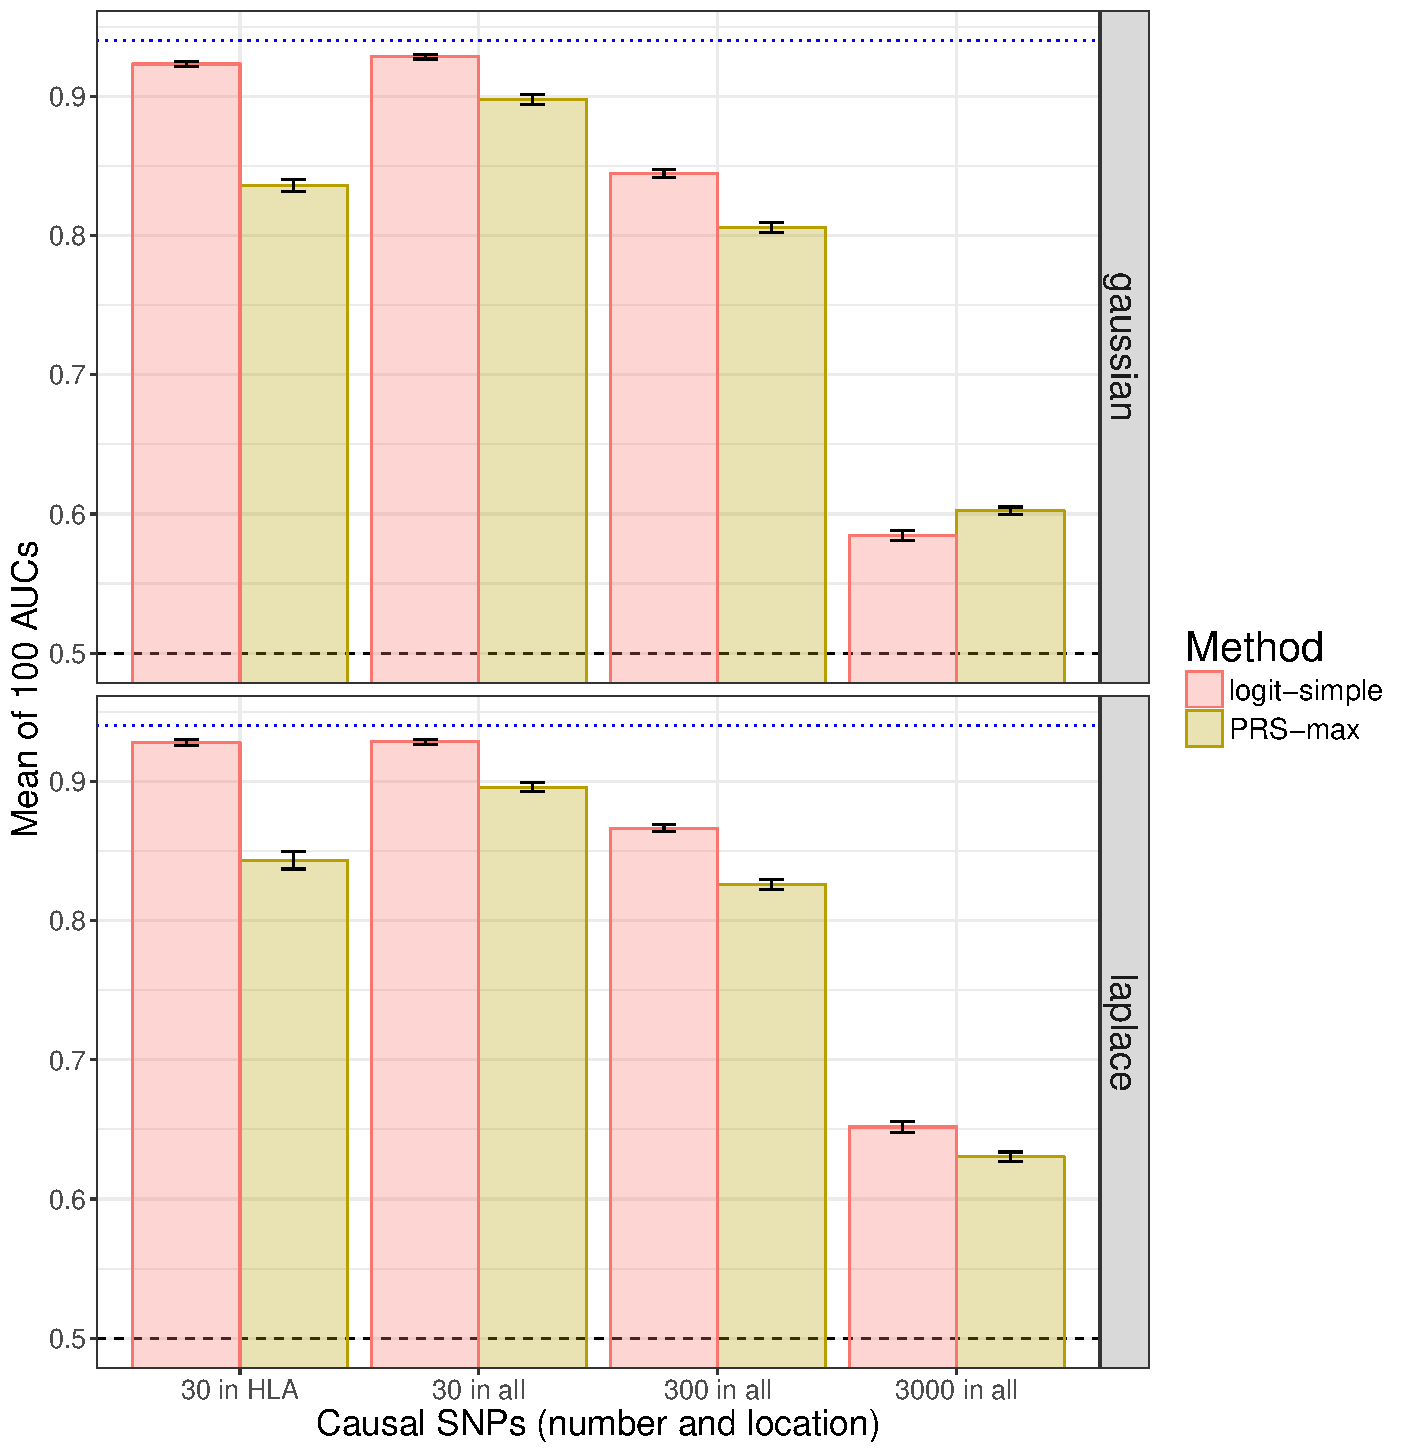
\includegraphics[width=\textwidth]{main-AUC-logit}}
\caption{Main comparison of the C+T and ``logit-simple'' methods in scenario \textnumero1 for the ``simple'' model and an heritability of 80\%. Mean of AUC over 100 simulations for ``logit-simple'' and the maximum AUC reported with the C+T method (``PRS-max''). Upper (lower) panel is presenting results for effets following a Gaussian (Laplace) distribution. Error bars are representing $\pm 2 \text{SD}$ of $10^5$ non-parametric bootstrap of the mean of AUC. The blue dotted line represents the maximum achievable AUC.}
\label{fig:main-AUC-logit}
\end{figure}

\newpage
\begin{figure}[h]
\centerline{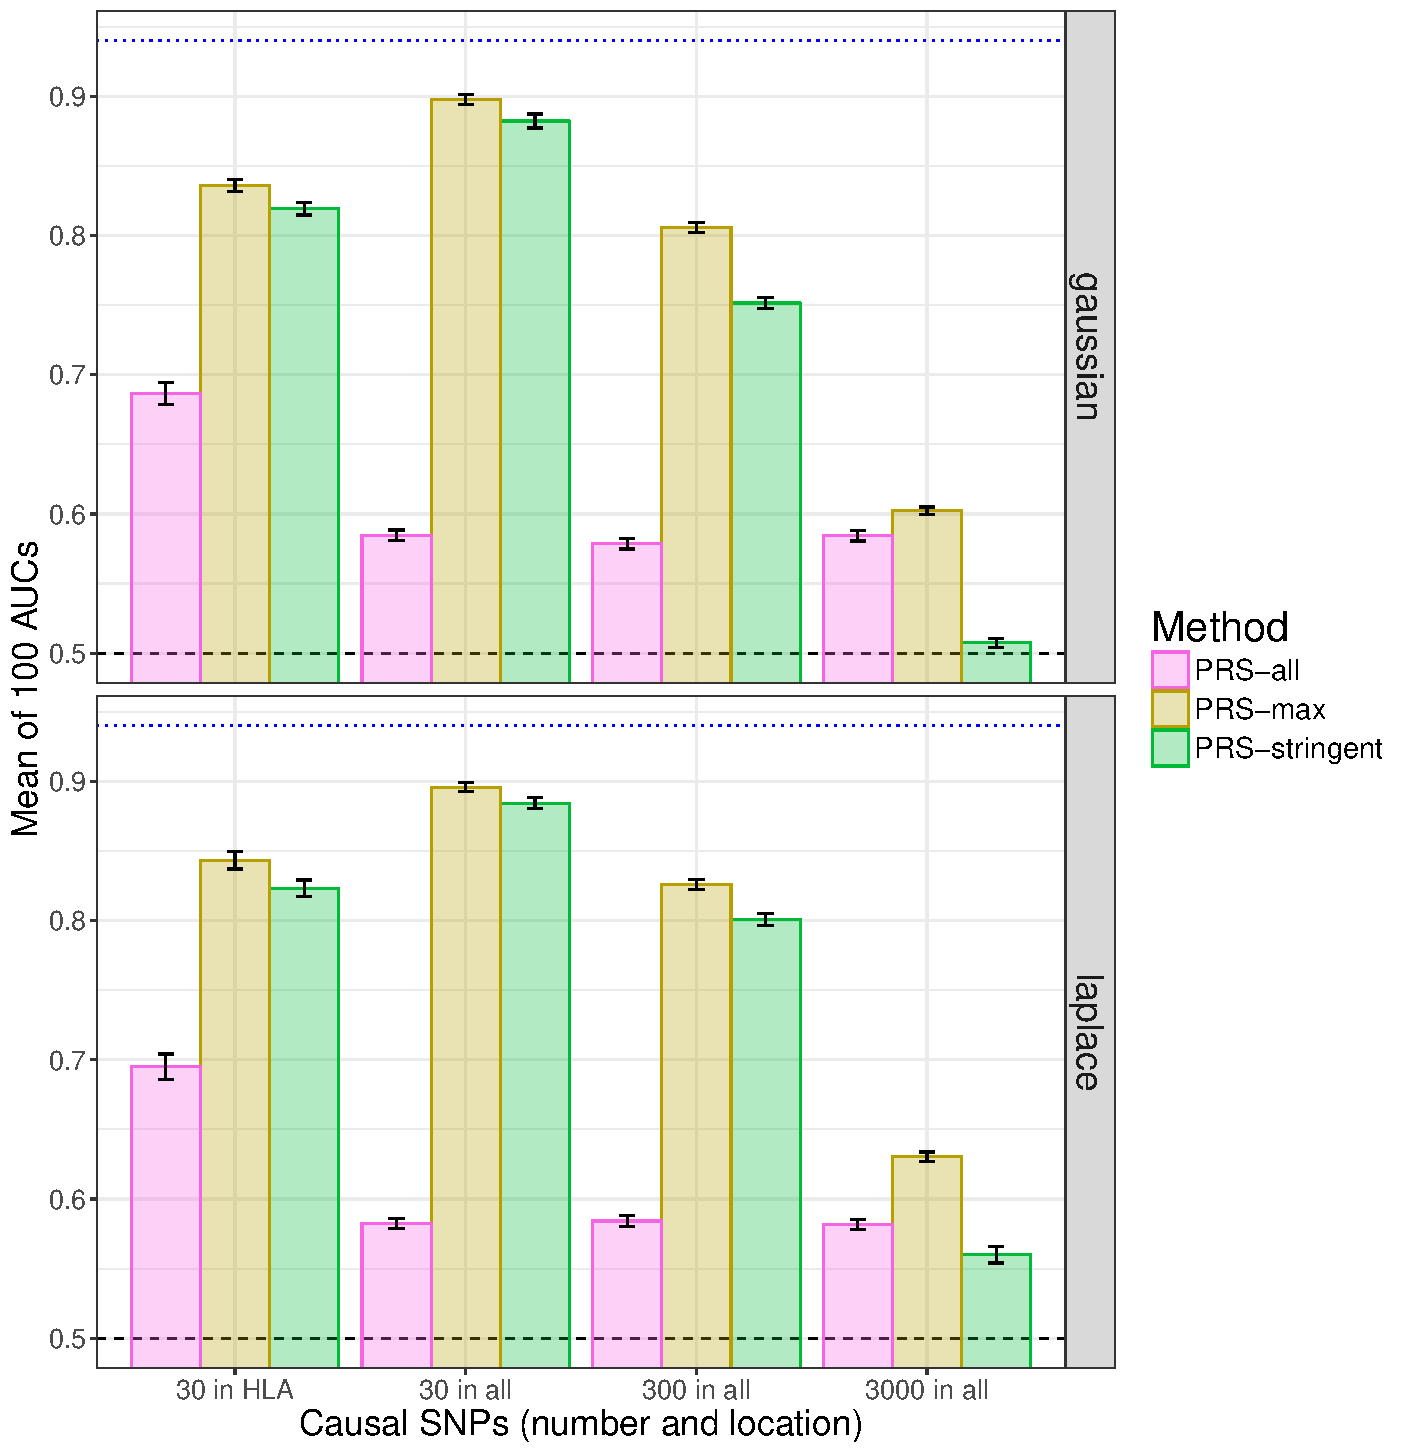
\includegraphics[width=\textwidth]{main-AUC-PRS}}
\caption{Comparison of three different p-value thresholds used in the C+T method in scenario \textnumero1 for the ``simple'' model and an heritability of 80\%. Mean of AUC over 100 simulations. Upper (lower) panel is presenting results for effets following a Gaussian (Laplace) distribution. Error bars are representing $\pm 2 \text{SD}$ of $10^5$ non-parametric bootstrap of the mean of AUC. The blue dotted line represents the maximum achievable AUC.}
\label{fig:main-AUC-PRS}
\end{figure}

\newpage
\begin{figure}[h]
\centerline{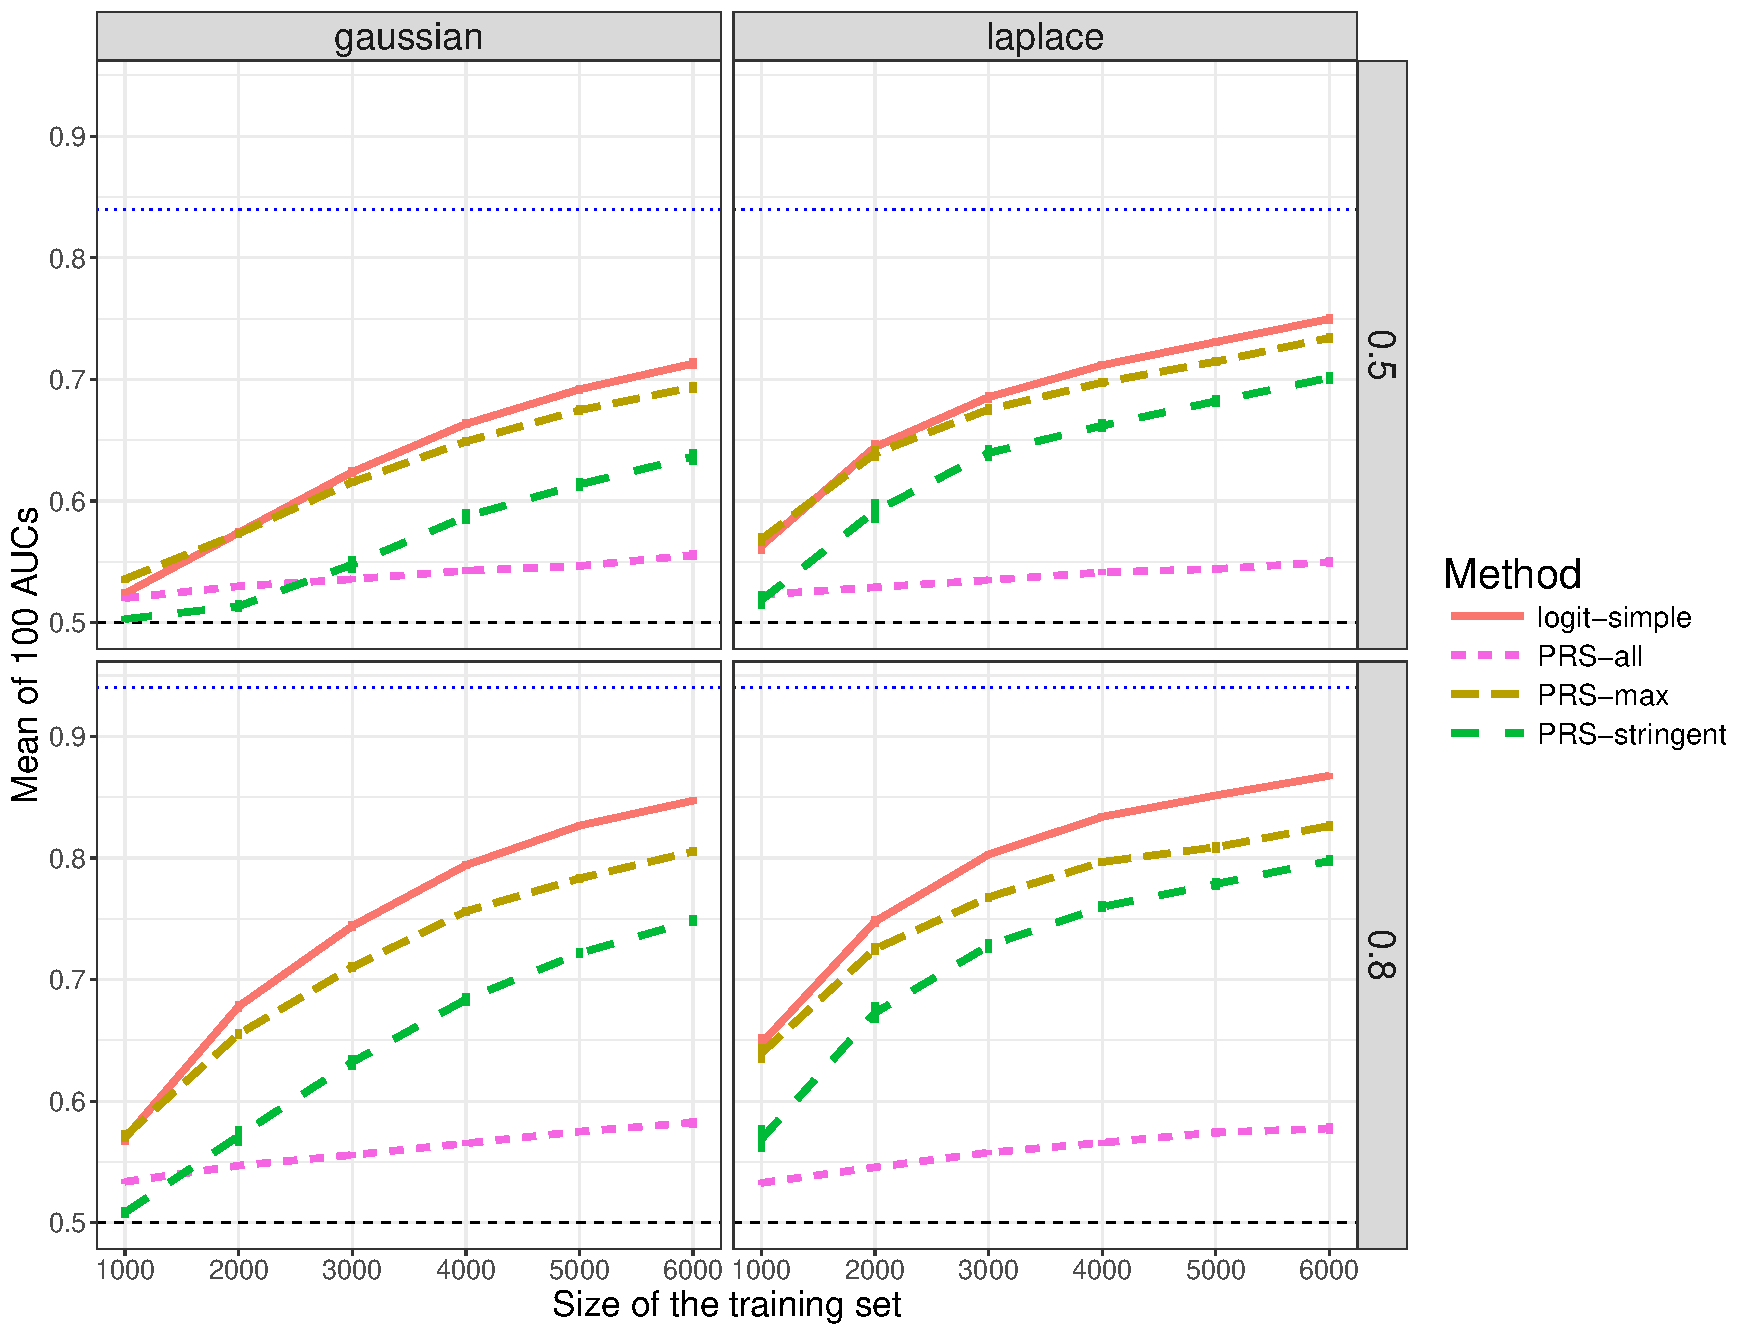
\includegraphics[width=\textwidth]{main-AUC-ntrain}}
\caption{Comparison of models when varying sample size in scenario \textnumero3 for the ``simple'' model with 300 causal SNPs sampled anywhere on the genome. Mean of AUC over 100 simulations for the maximum values of PRS for three different $r^2$ thresholds ($0.05$, $0.2$ and $0.8$) and ``logit-simple'' as a function of the training size. Upper (lower) panels are presenting results for effets following a Gaussian (Laplace) distribution and left (right) panels are presenting results for an heritability of 0.5 (0.8). Error bars are representing $\pm 2 \text{SD}$ of $10^5$ non-parametric bootstrap of the mean of AUC. The blue dotted line represents the maximum achievable AUC.}
\label{fig:main-AUC-ntrain}
\end{figure}

\newpage
\begin{figure}[h]
\centerline{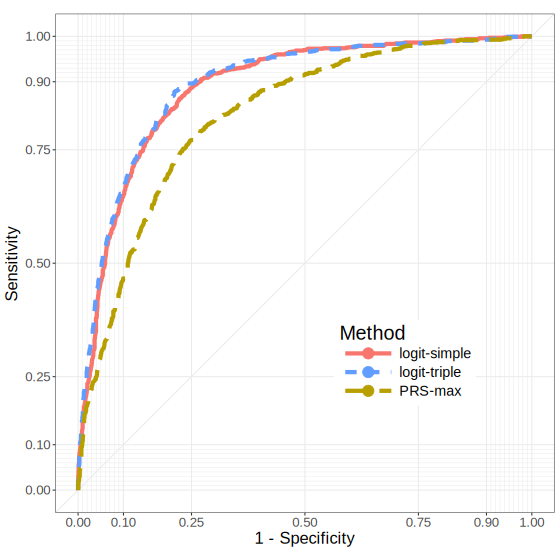
\includegraphics[width=\textwidth]{celiac-roc}}
\caption{ROC Curves for the ``C+T'', ``logit-simple'' and ``logit-triple'' methods for Celiac disease dataset. Models were trained using 12,000 individuals. These are results projecting these models on the remaining 3155 individuals. The figure is plotted using R package plotROC \cite[]{sachs2017plotroc}.\label{fig:celiac-roc}}
\end{figure}

%%%%%%%%%%%%%%%%%%%%%%%%%%%%%%%%%%%%%%%%%%%%%%%%%%%%%%%%%%%%%%%%%%%%%%%%%%%%%%%%

\clearpage
\section*{Acknowledgements}

Authors acknowledge LabEx PERSYVAL-Lab (ANR-11-LABX-0025-01). Authors also acknowledge the Grenoble Alpes Data Institute that is supported by the French National Research Agency under the ``Investissements d'avenir'' program (ANR-15-IDEX-02).
We are also grateful to F\'elix Balazard for useful discussions about T-Trees, and to Yaohui Zeng for useful discussions about R package biglasso.

\vspace*{-12pt}

\bibliographystyle{natbib}
\bibliography{refs}

%%%%%%%%%%%%%%%%%%%%%%%%%%%%%%%%%%%%%%%%%%%%%%%%%%%%%%%%%%%%%%%%%%%%%%%%%%%%%%%%
%%%%%%%%%%%%%%%%%%%%%%%%%%%%%%%%%%%%%%%%%%%%%%%%%%%%%%%%%%%%%%%%%%%%%%%%%%%%%%%%
%%%%%%%%%%%%%%%%%%%%%%%%%%%%%%%%%%%%%%%%%%%%%%%%%%%%%%%%%%%%%%%%%%%%%%%%%%%%%%%%

\newpage
\section*{Supplementary Materials}

\renewcommand{\thefigure}{S\arabic{figure}}
\setcounter{figure}{0}
\renewcommand{\thetable}{S\arabic{table}}
\setcounter{table}{0}

%%%%%%%%%%%%%%%%%%%%%%%%%%%%%%%%%%%%%%%%%%%%%%%%%%%%%%%%%%%%%%%%%%%%%%%%%%%%%%%%

\subsection*{``Fancy'' model}

For the ``fancy'' model, we separate the causal SNPs in three equal sets $S_\text{causal}^{(1)}$, $S_\text{causal}^{(2)}$
and $S_\text{causal}^{(3)}$; $S_\text{causal}^{(3)}$ is further separated in two equal sets, $S_\text{causal}^{(3.1)}$ and $S_\text{causal}^{(3.2)}$.
We then compute $$y_i = \underbrace{\sum_{j\in S_\text{causal}^{(1)}} w_j \cdot \widetilde{G_{i,j}}}_\text{linear} + \underbrace{\sum_{j\in S_\text{causal}^{(2)}} w_j \cdot \widetilde{D_{i,j}}}_\text{dominant} + \underbrace{\sum_{\substack{k=1 \\ j_1=e_k^{(3.1)} \\ j_2=e_k^{(3.2)}}}^{k=\left|S_\text{causal}^{(3.1)}\right|} w_{j_1} \cdot \widetilde{G_{i,j_1} G_{i,j_2}}}_\text{interaction} ~~+~~ \epsilon_i~,$$
where $D_{i,j} = \mathds{1}\left\{G_{i,j} \neq 0\right\}$ and $S_\text{causal}^{(q)}=\left\{e_k^{(q)},~k \in \left\{1, \ldots, \left|S_\text{causal}^{(q)}\right|\right\}\right\}$.
%Note that, because we use the raw genotype counts when coding the interaction terms, the corresponding SNPs also display a marginal effect.

\subsection*{Maximum AUCs} \label{sec:auc-max}

We used three different ways to estimate the maximum achievable AUC for our simulations.
First, we used the estimation from equation (3) of \cite{wray2010genetic}. For a prevalence fixed at 30\% and an heritability of 50\% (respectively 80\%), the approximated theoretical values of AUC are 84.1\% (respectively 93.0\%). Note that this approximation is reported to be less accurate for high heritabilities.
Secondly, if we assume that the genetic part of the liabilities follows a Gaussian distribution $N(0, h^2)$ and that the environmental part follows a Gaussian distribution $N(0, 1 - h^2)$, we can estimate the theoretical value of the AUC that can be achieved given the disease heritability $h^2$ through Monte Carlo simulations. We report AUCs of 84.1\% and 94.1\% for an heritability of 50\% and 80\%, respectively.
Thirdly, we reproduce the exact same procedure of simulations and, for each combination of parameters (Table \ref{tab:simus}), we estimate the AUC of the ``oracle'', i.e.\ the true simulated genetic part of the liabilities through 100 replicates. For every combination of parameters, AUC of oracles are comprised between 83.2\% and 84.2\% for an heritability of 50\% and between 93.2\% and 94.1\% for an heritability of 80\%.
Given all these estimates of the maximal achievable AUC and for the sake of simplicity, we report maximum AUCs of 84\% (94\%) for heritabilities of 50\% (80\%) whatever are the parameters of the simulations.


%%%%%%%%%%%%%%%%%%%%%%%%%%%%%%%%%%%%%%%%%%%%%%%%%%%%%%%%%%%%%%%%%%%%%%%%%%%%%%%%

\newpage

\begin{table}[ht]
\centering
\begin{tabular}{|l|cccc|r|}
\hline
Population & UK & Finland & Netherlands & Italy & Total\\
\hline
Cases & 2569 & 637 & 795 & 495 & 4496\\
Controls & 7492 & 1799 & 828 & 540 & 10659\\
\hline
Total & 10061 & 2436 & 1623 & 1035 & 15155\\
\hline
\end{tabular}
\caption{Number of individuals by population and disease status in the celiac disease case-control study (after quality control, genotyped on 281,122 SNPs).\label{tab:celiac-data}}
\end{table}

%%%%%%%%%%%%%%%%%%%%%%%%%%%%%%%%%%%%%%%%%%%%%%%%%%%%%%%%%%%%%%%%%%%%%%%%%%%%%%%%

% latex table generated in R 3.4.1 by xtable 1.8-2 package
% Thu Oct 26 16:46:26 2017
\begin{table}[ht]
\centering
\begin{tabular}{ccccccccccccccc}
  \hline
1.00e+00 & 7.22e-01 & 5.87e-01 & 4.20e-01 & 2.43e-01 & 1.00e-01 & 2.35e-02 & 2.21e-03 & 4.69e-05 & 8.81e-08 & 3.18e-12 & 1.83e-19 & 2.89e-31 & 1.70e-50 & 7.71e-82 \\ 
  5.00e-08 & 7.05e-01 & 5.65e-01 & 3.95e-01 & 2.20e-01 & 8.47e-02 & 1.79e-02 & 1.42e-03 & 2.28e-05 & 2.73e-08 & 4.69e-13 & 8.08e-21 & 1.80e-33 & 4.30e-54 & 1.06e-87 \\ 
  7.94e-01 & 6.87e-01 & 5.42e-01 & 3.69e-01 & 1.97e-01 & 7.08e-02 & 1.34e-02 & 8.83e-04 & 1.05e-05 & 7.74e-09 & 6.03e-14 & 2.86e-22 & 7.73e-36 & 5.97e-58 & 5.49e-94 \\ 
  7.81e-01 & 6.69e-01 & 5.19e-01 & 3.43e-01 & 1.75e-01 & 5.85e-02 & 9.79e-03 & 5.31e-04 & 4.61e-06 & 2.01e-09 & 6.69e-15 & 7.92e-24 & 2.24e-38 & 4.37e-62 & 1.00e-100 \\ 
  7.67e-01 & 6.50e-01 & 4.95e-01 & 3.18e-01 & 1.54e-01 & 4.76e-02 & 7.01e-03 & 3.08e-04 & 1.90e-06 & 4.72e-10 & 6.32e-16 & 1.70e-25 & 4.26e-41 & 1.61e-66 &  \\ 
  7.53e-01 & 6.30e-01 & 4.70e-01 & 2.93e-01 & 1.35e-01 & 3.82e-02 & 4.90e-03 & 1.72e-04 & 7.31e-07 & 1.00e-10 & 5.04e-17 & 2.75e-27 & 5.16e-44 & 2.83e-71 &  \\ 
  7.38e-01 & 6.09e-01 & 4.46e-01 & 2.68e-01 & 1.17e-01 & 3.02e-02 & 3.33e-03 & 9.18e-05 & 2.63e-07 & 1.89e-11 & 3.35e-18 & 3.31e-29 & 3.84e-47 & 2.26e-76 &  \\ 
   \hline
\end{tabular}
\caption{The 102 thresholds used for the C+T method for this study.\label{tab:thr}}
\end{table}

%%%%%%%%%%%%%%%%%%%%%%%%%%%%%%%%%%%%%%%%%%%%%%%%%%%%%%%%%%%%%%%%%%%%%%%%%%%%%%%%

\newpage
\begin{figure}[h]
\centerline{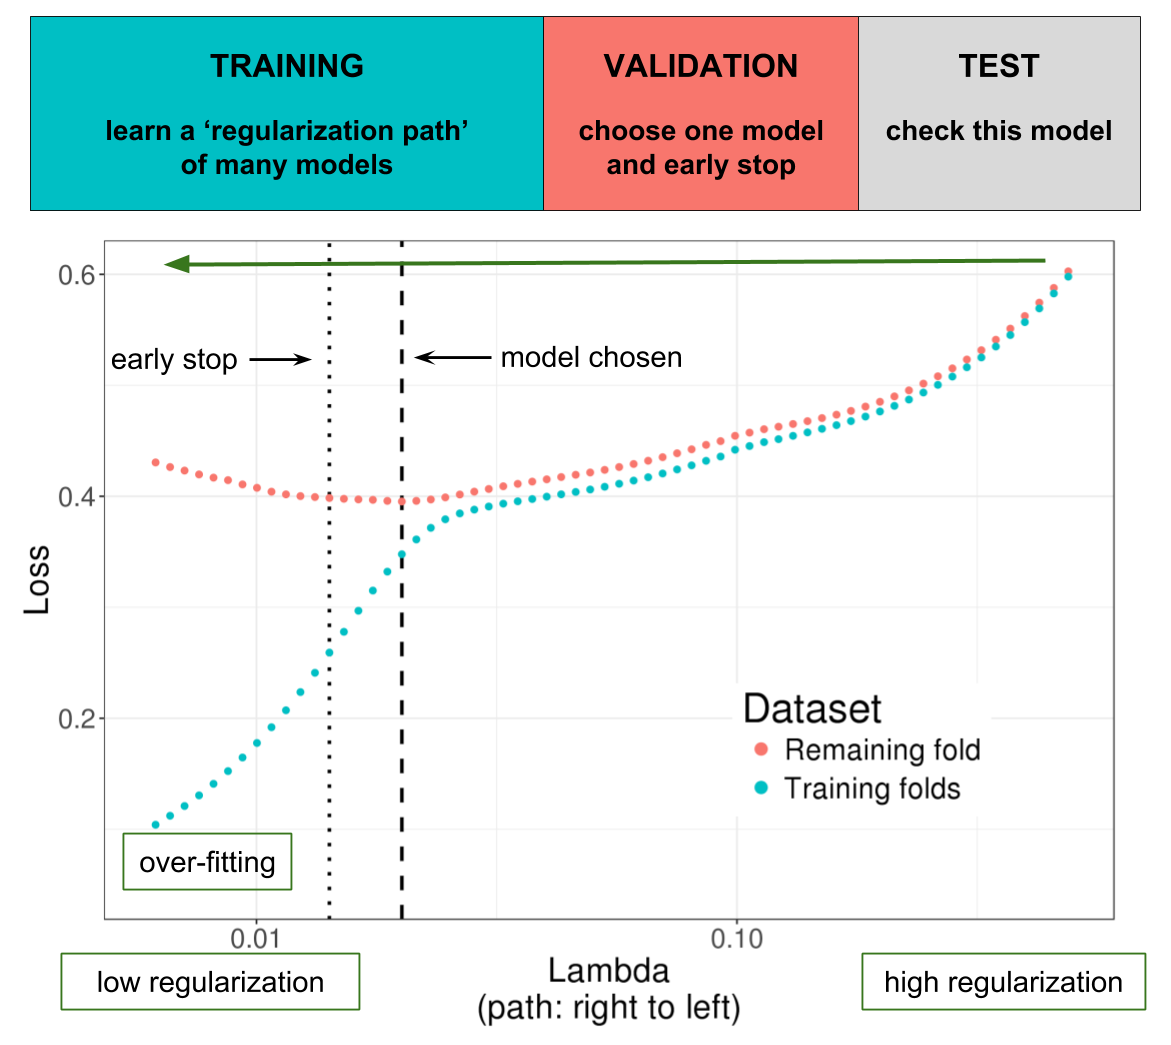
\includegraphics[width=\textwidth]{simple-CMSA}}
\caption{Illustration of one turn of the Cross-Model Selection and Averaging (CMSA) procedure. First, this procedure separates the training set in $K$ folds (e.g.\ 10 folds). 
Secondly, in turn, each fold is considered as an inner validation set (red) and the other ($K - 1$) folds form an inner training set (blue). A ``regularization path'' of models is trained on the inner training set and the corresponding predictions (scores) for the inner validation set are computed. The model that minimizes the loss on the inner validation set is selected. Finally, the $K$ resulting models are averaged. 
We also use this procedure to derive an early stopping criterion so that the algorithm does not need to evaluate the whole regularization paths, making this procedure much faster.}
\label{fig:CMSA}
\end{figure}

%%%%%%%%%%%%%%%%%%%%%%%%%%%%%%%%%%%%%%%%%%%%%%%%%%%%%%%%%%%%%%%%%%%%%%%%%%%%%%%%

\newpage
\begin{figure}[h]
\centerline{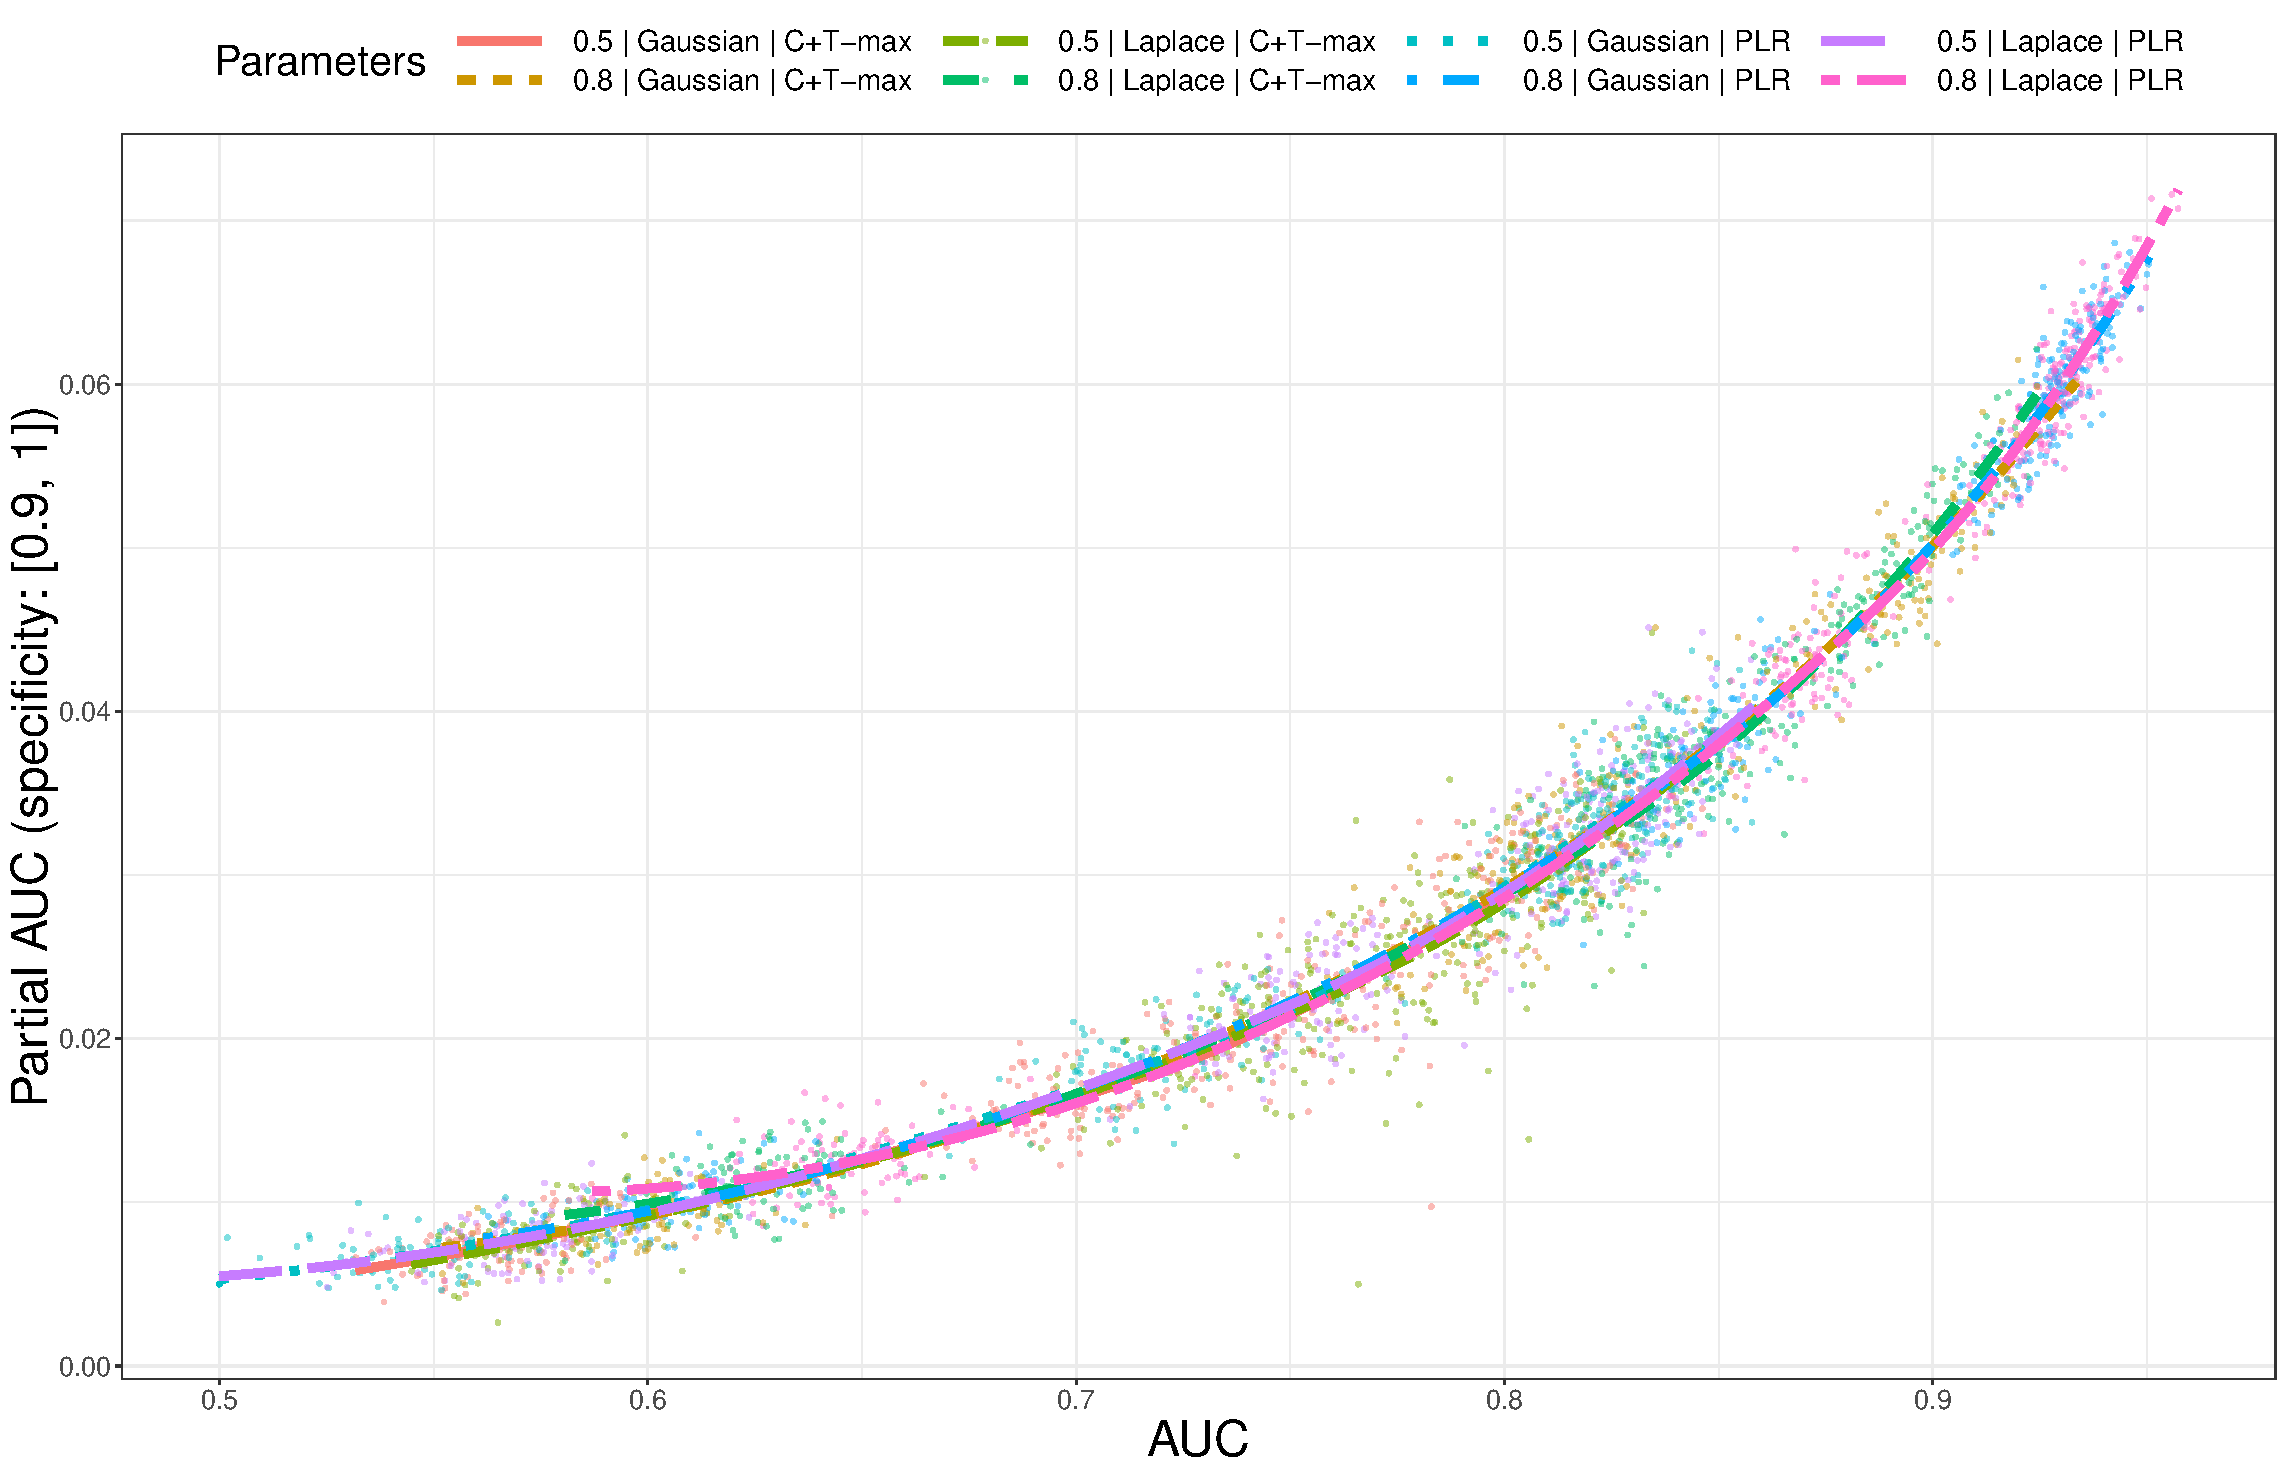
\includegraphics[width=\textwidth]{supp-AUC-corr}}
\caption{Correlation between AUC and partial AUC values in scenario \textnumero1. There is a Spearman correlation of 98\% between values of AUC and partial AUC. The relation between the two values are the same whatever are the disease heritability, distribution of effects and method used.\label{fig:supp-AUC-corr}}
\end{figure}

%%%%%%%%%%%%%%%%%%%%%%%%%%%%%%%%%%%%%%%%%%%%%%%%%%%%%%%%%%%%%%%%%%%%%%%%%%%%%%%%

\newpage
\begin{figure}[h]
\centerline{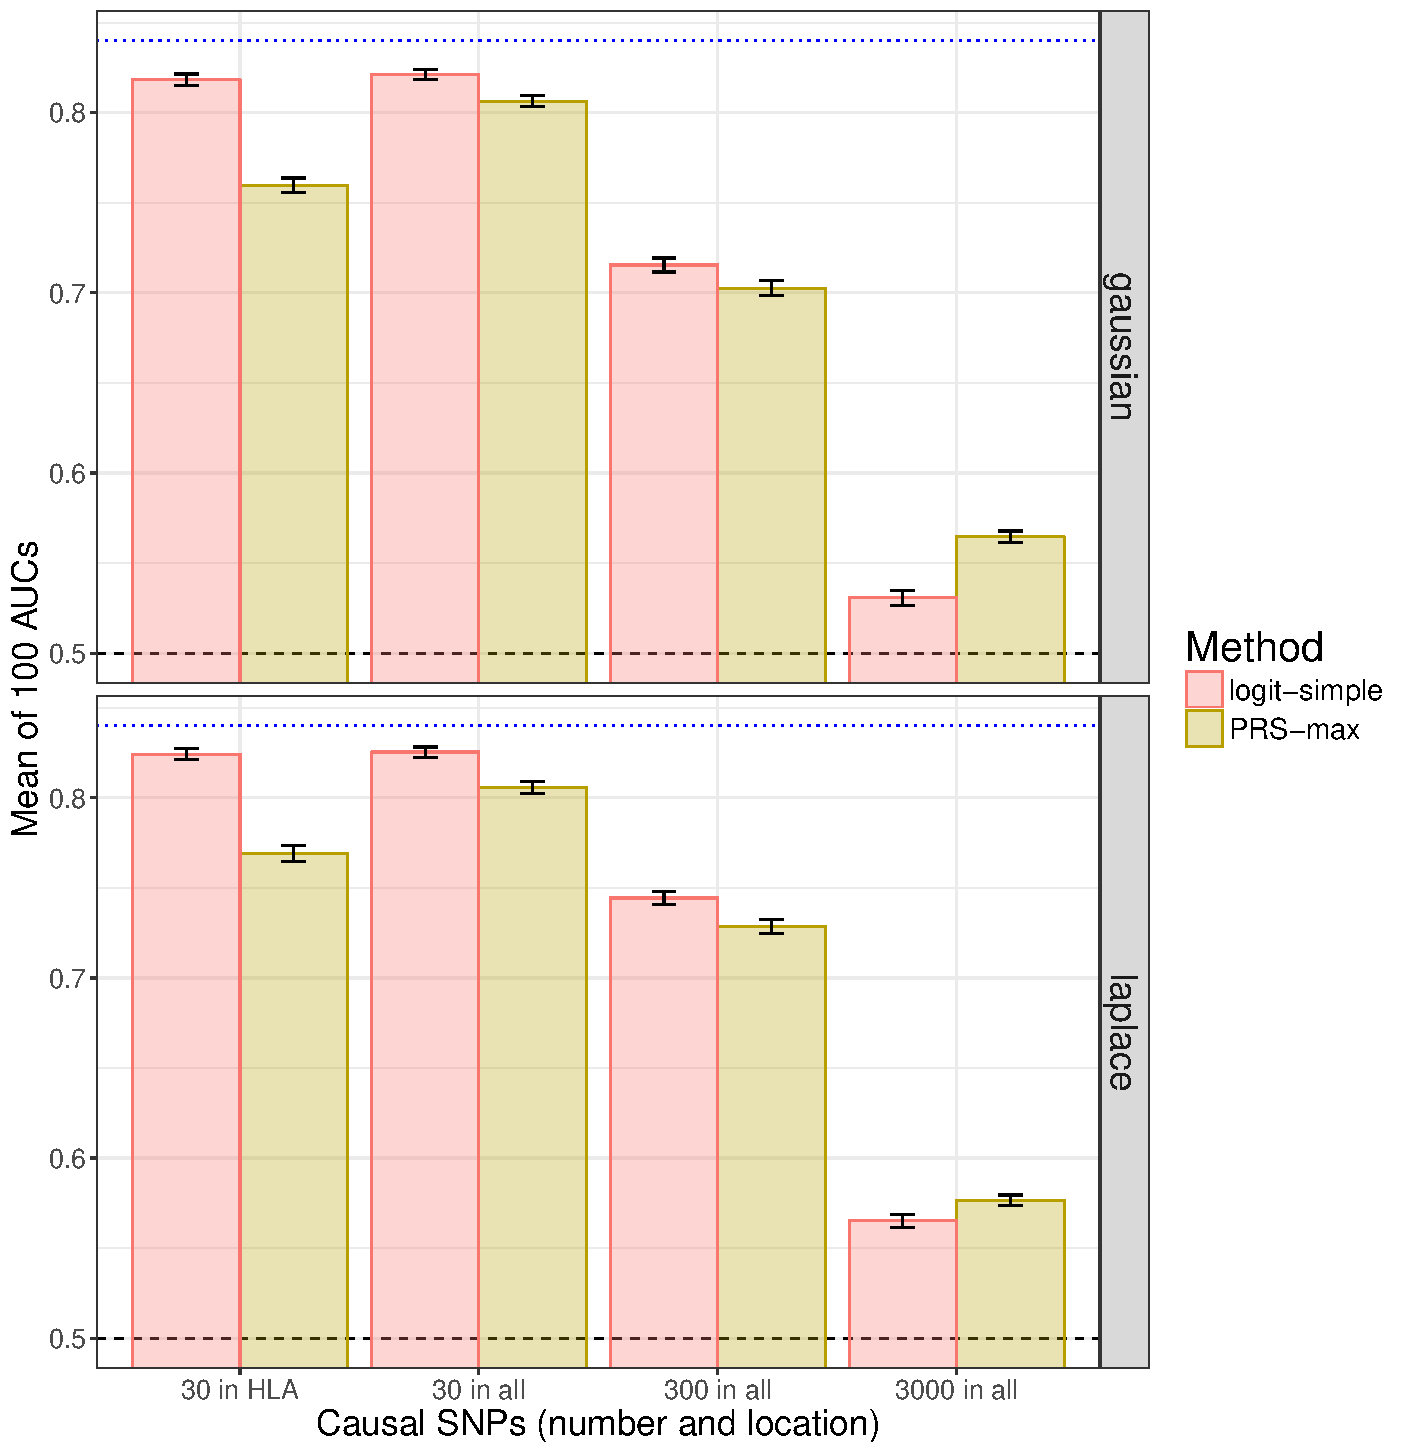
\includegraphics[width=\textwidth]{supp-AUC-logit}}
\caption{Comparison of the C+T and ``logit-simple'' methods in scenario \textnumero1 for the ``simple'' model and an heritability of 50\%. Mean of AUC over 100 simulations for ``logit-simple'' and the maximum AUC reported with the C+T method (``PRS-max''). Upper (lower) panel is presenting results for effets following a Gaussian (Laplace) distribution. Error bars are representing $\pm 2 \text{SD}$ of $10^5$ non-parametric bootstrap of the mean of AUC. The blue dotted line represents the maximum achievable AUC.}
\label{fig:supp-AUC-logit}
\end{figure}

\newpage
\begin{figure}[h]
\centerline{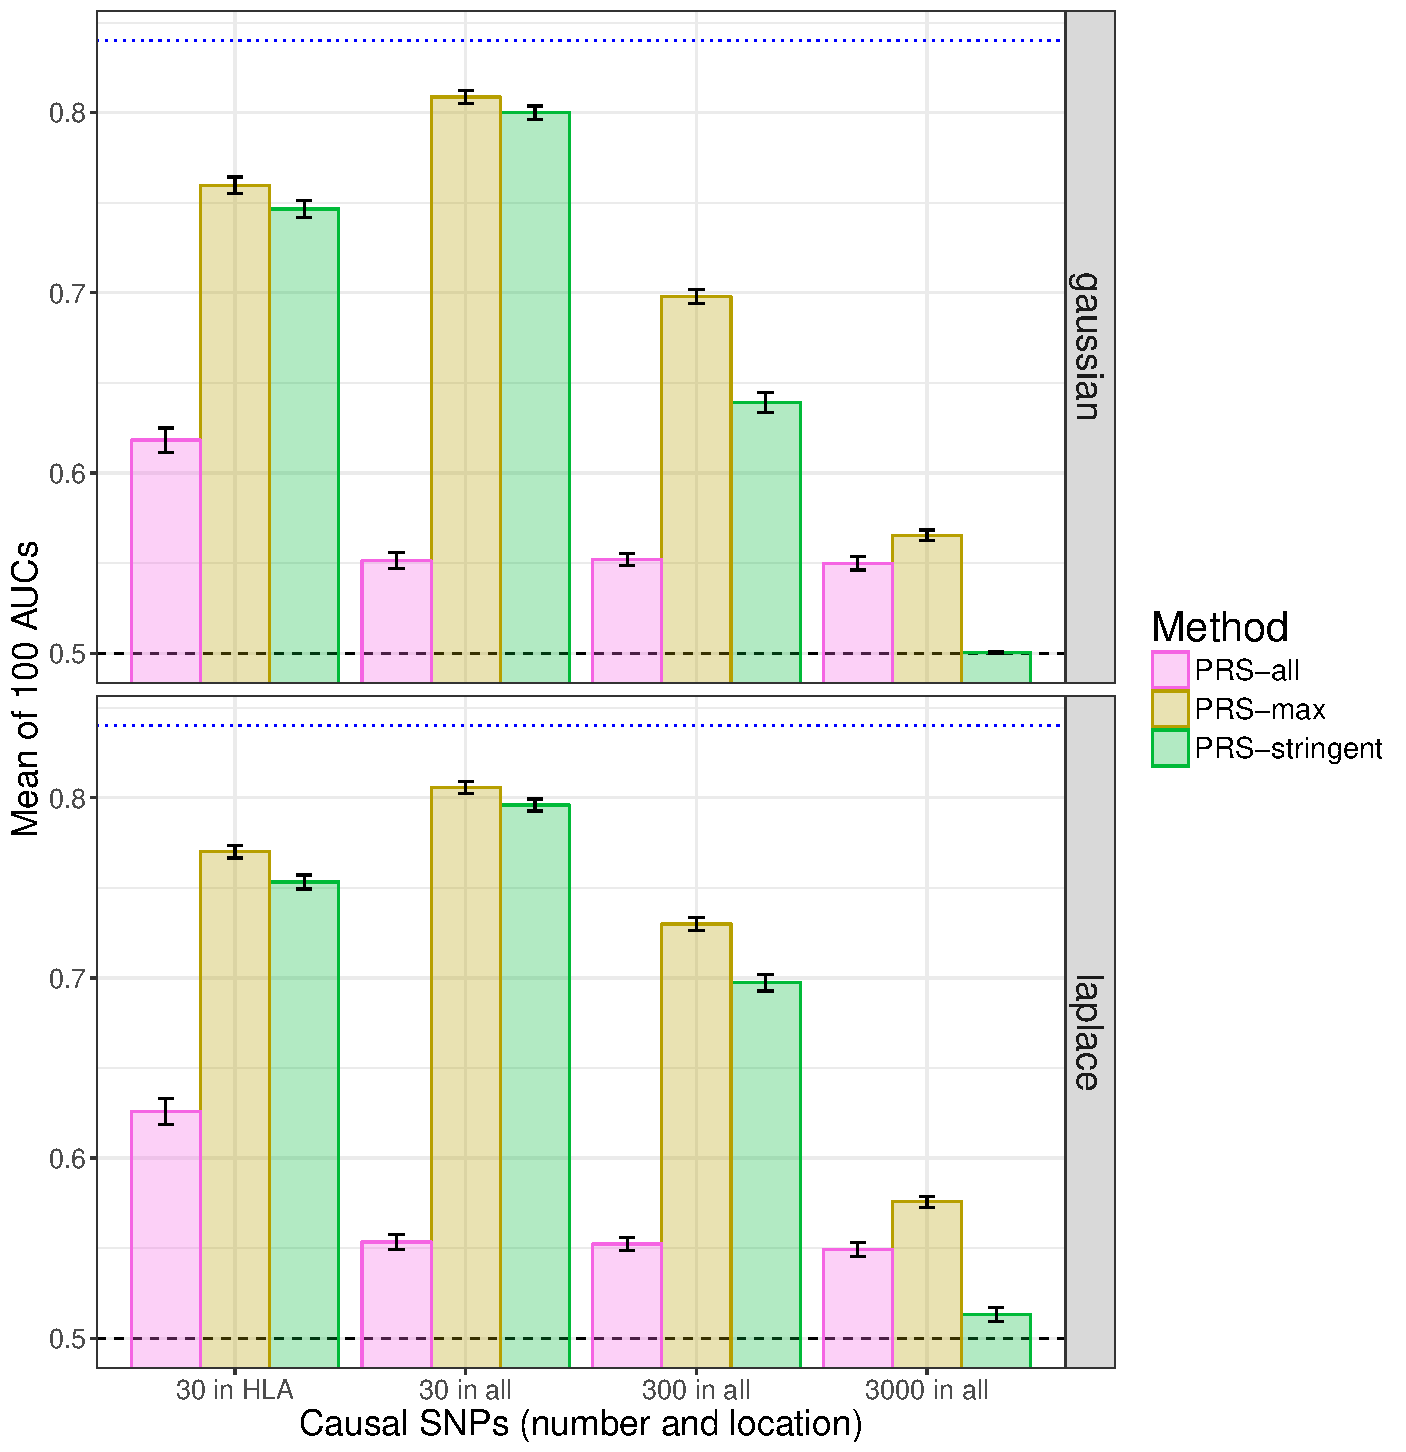
\includegraphics[width=\textwidth]{supp-AUC-PRS}}
\caption{Comparison of three different p-value thresholds used in the C+T method in scenario \textnumero1 for the ``simple'' model and an heritability of 50\%. Mean of AUC over 100 simulations. Upper (lower) panel is presenting results for effets following a Gaussian (Laplace) distribution. Error bars are representing $\pm 2 \text{SD}$ of $10^5$ non-parametric bootstrap of the mean of AUC. The blue dotted line represents the maximum achievable AUC.}
\label{fig:supp-AUC-PRS}
\end{figure}

\newpage
\begin{figure}[h]
\centerline{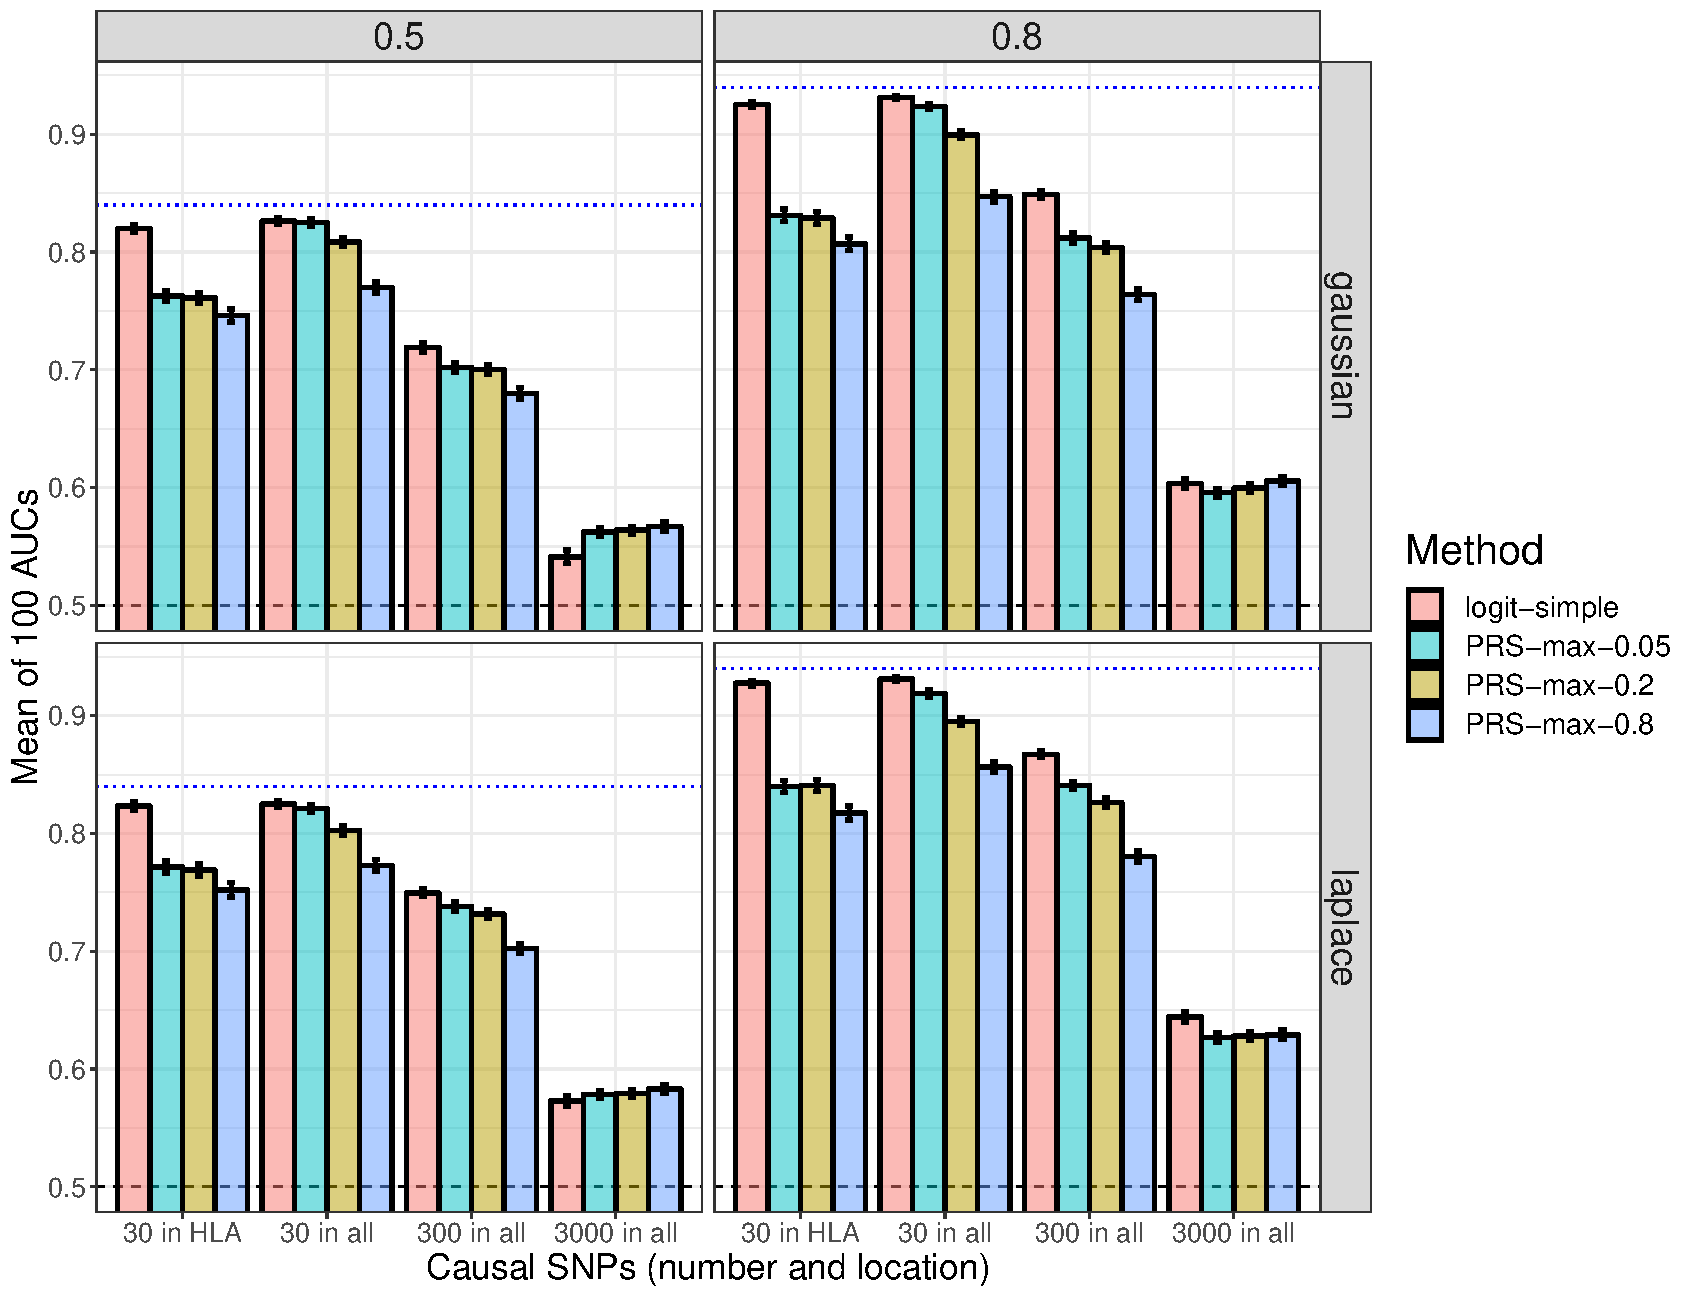
\includegraphics[width=\textwidth]{supp-AUC-all-r2}}
\caption{Comparison of models in scenario \textnumero1 for the ``simple'' model. Mean of AUC over 100 simulations for the maximum values of PRS for three different $r^2$ thresholds ($0.05$, $0.2$ and $0.8$) and ``logit-simple'' as a function of the number and location of causal SNPs. Upper (lower) panels are presenting results for effets following a Gaussian (Laplace) distribution and left (right) panels are presenting results for an heritability of 0.5 (0.8). Error bars are representing $\pm 2 \text{SD}$ of $10^5$ non-parametric bootstrap of the mean of AUC. The blue dotted line represents the maximum achievable AUC.}
\label{fig:supp-AUC-all-r2}
\end{figure}

\newpage
\begin{figure}[h]
\centerline{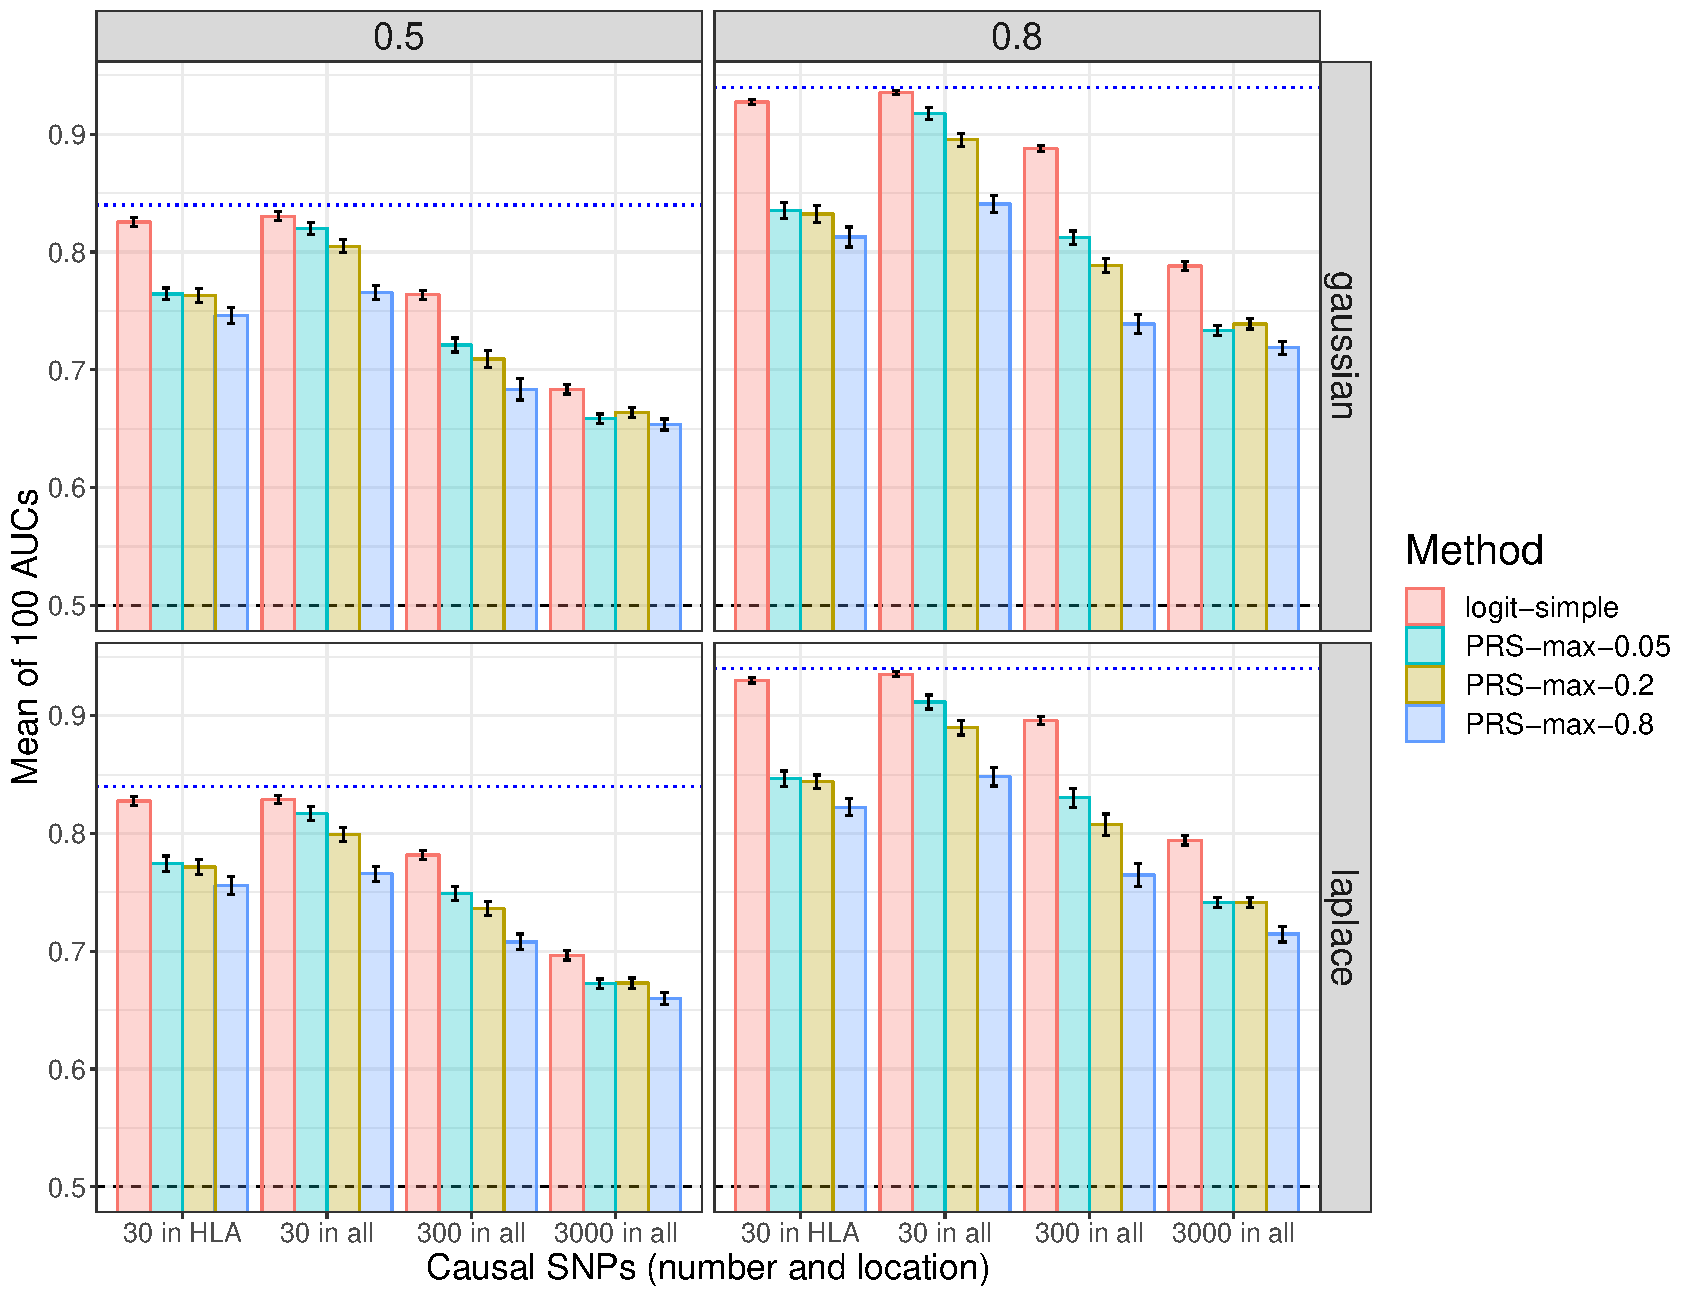
\includegraphics[width=\textwidth]{supp-AUC-chr6-all-r2}}
\caption{Comparison of models in scenario \textnumero2 (using chromosome 6 only) for the ``simple'' model. Thinner lines represents results in scenario \textnumero1 (Figure \ref{fig:supp-AUC-all-r2}). Mean of AUC over 100 simulations for the maximum values of PRS for three different $r^2$ thresholds ($0.05$, $0.2$ and $0.8$) and ``logit-simple'' as a function of the number and location of causal SNPs. Upper (lower) panels are presenting results for effets following a Gaussian (Laplace) distribution and left (right) panels are presenting results for an heritability of 0.5 (0.8). Error bars are representing $\pm 2 \text{SD}$ of $10^5$ non-parametric bootstrap of the mean of AUC. The blue dotted line represents the maximum achievable AUC.}
\label{fig:supp-AUC-chr6-all-r2}
\end{figure}

%%%%%%%%%%%%%%%%%%%%%%%%%%%%%%%%%%%%%%%%%%%%%%%%%%%%%%%%%%%%%%%%%%%%%%%%%%%%%%%%

\newpage
\begin{figure}[h]
\centerline{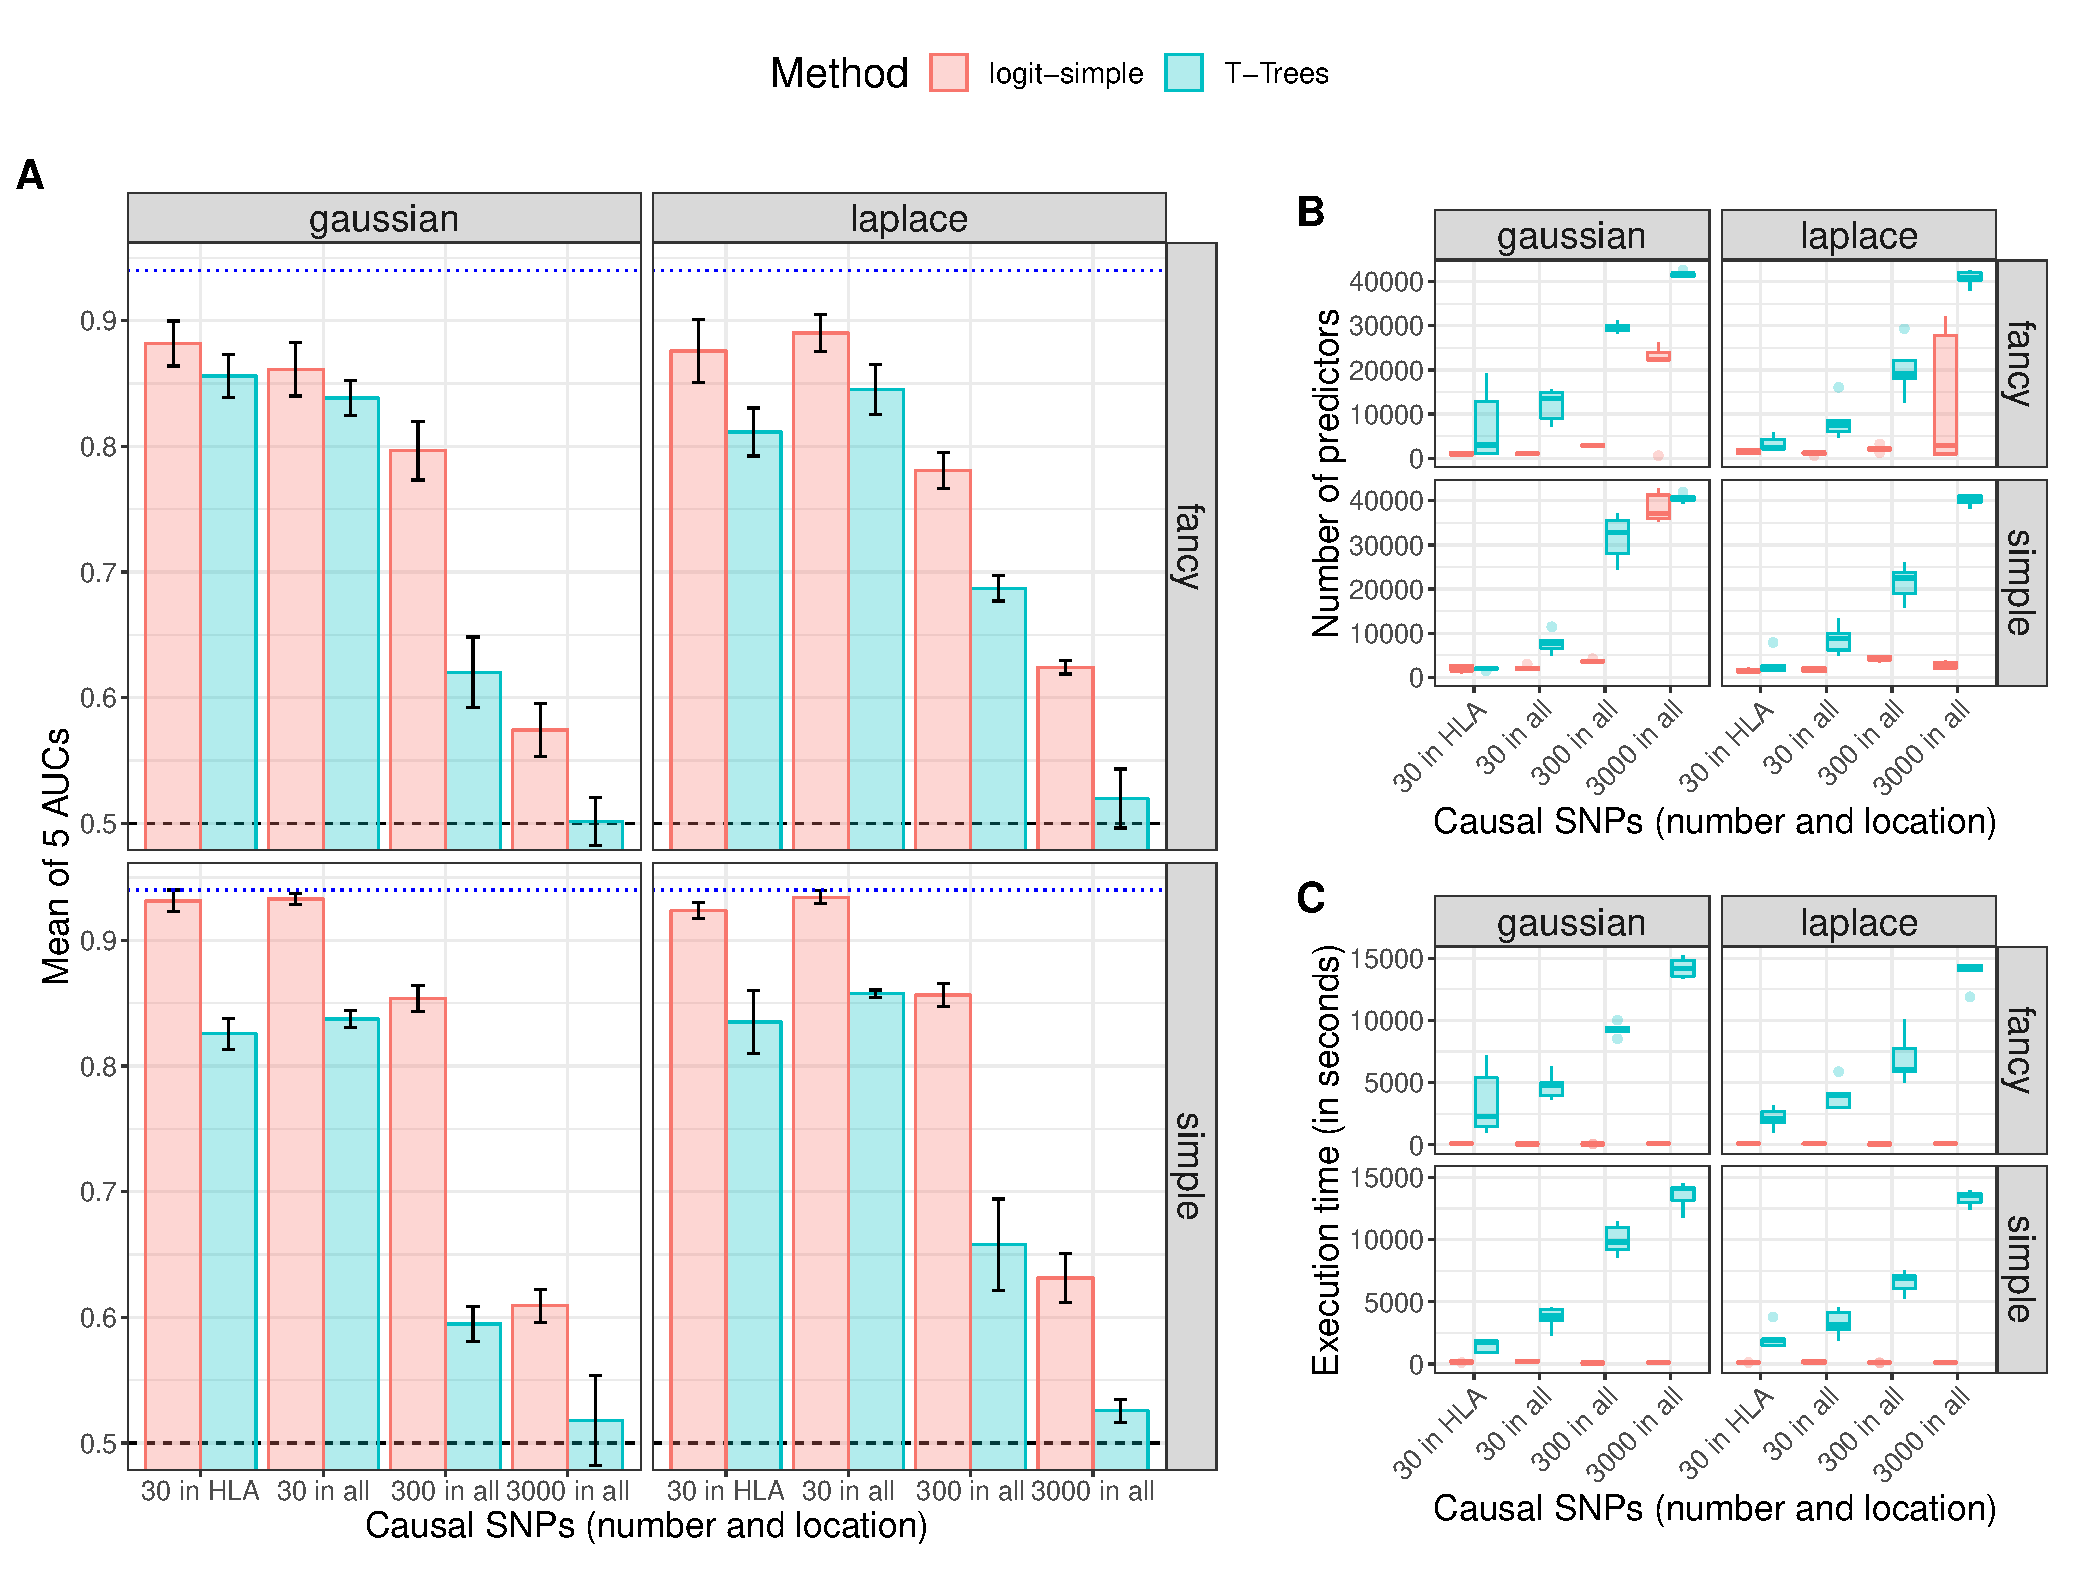
\includegraphics[width=\textwidth]{supp-ttrees}}
\caption{Comparison of T-Trees and ``logit-simple'' in scenario \textnumero1 for an heritability of 80\%. Vertical panels are presenting results for effects following a Gaussian or Laplace distribution. Horizontal panels are presenting results for the ``simple'' and ``fancy'' models for simulating phenotypes. \textbf{A:} Mean of AUC over 5 simulations. Error bars are representing $\pm 2 \text{SD}$ of $10^5$ non-parametric bootstrap of the mean of AUC. The blue dotted line represents the maximum achievable AUC. \textbf{B:} Boxplots of numbers of predictors used by the methods for 5 simulations. \textbf{C:} Boxplots of execution times for 5 simulations.}
\label{fig:supp-ttrees}
\end{figure}

%%%%%%%%%%%%%%%%%%%%%%%%%%%%%%%%%%%%%%%%%%%%%%%%%%%%%%%%%%%%%%%%%%%%%%%%%%%%%%%%

\newpage
\begin{figure}[h]
\centerline{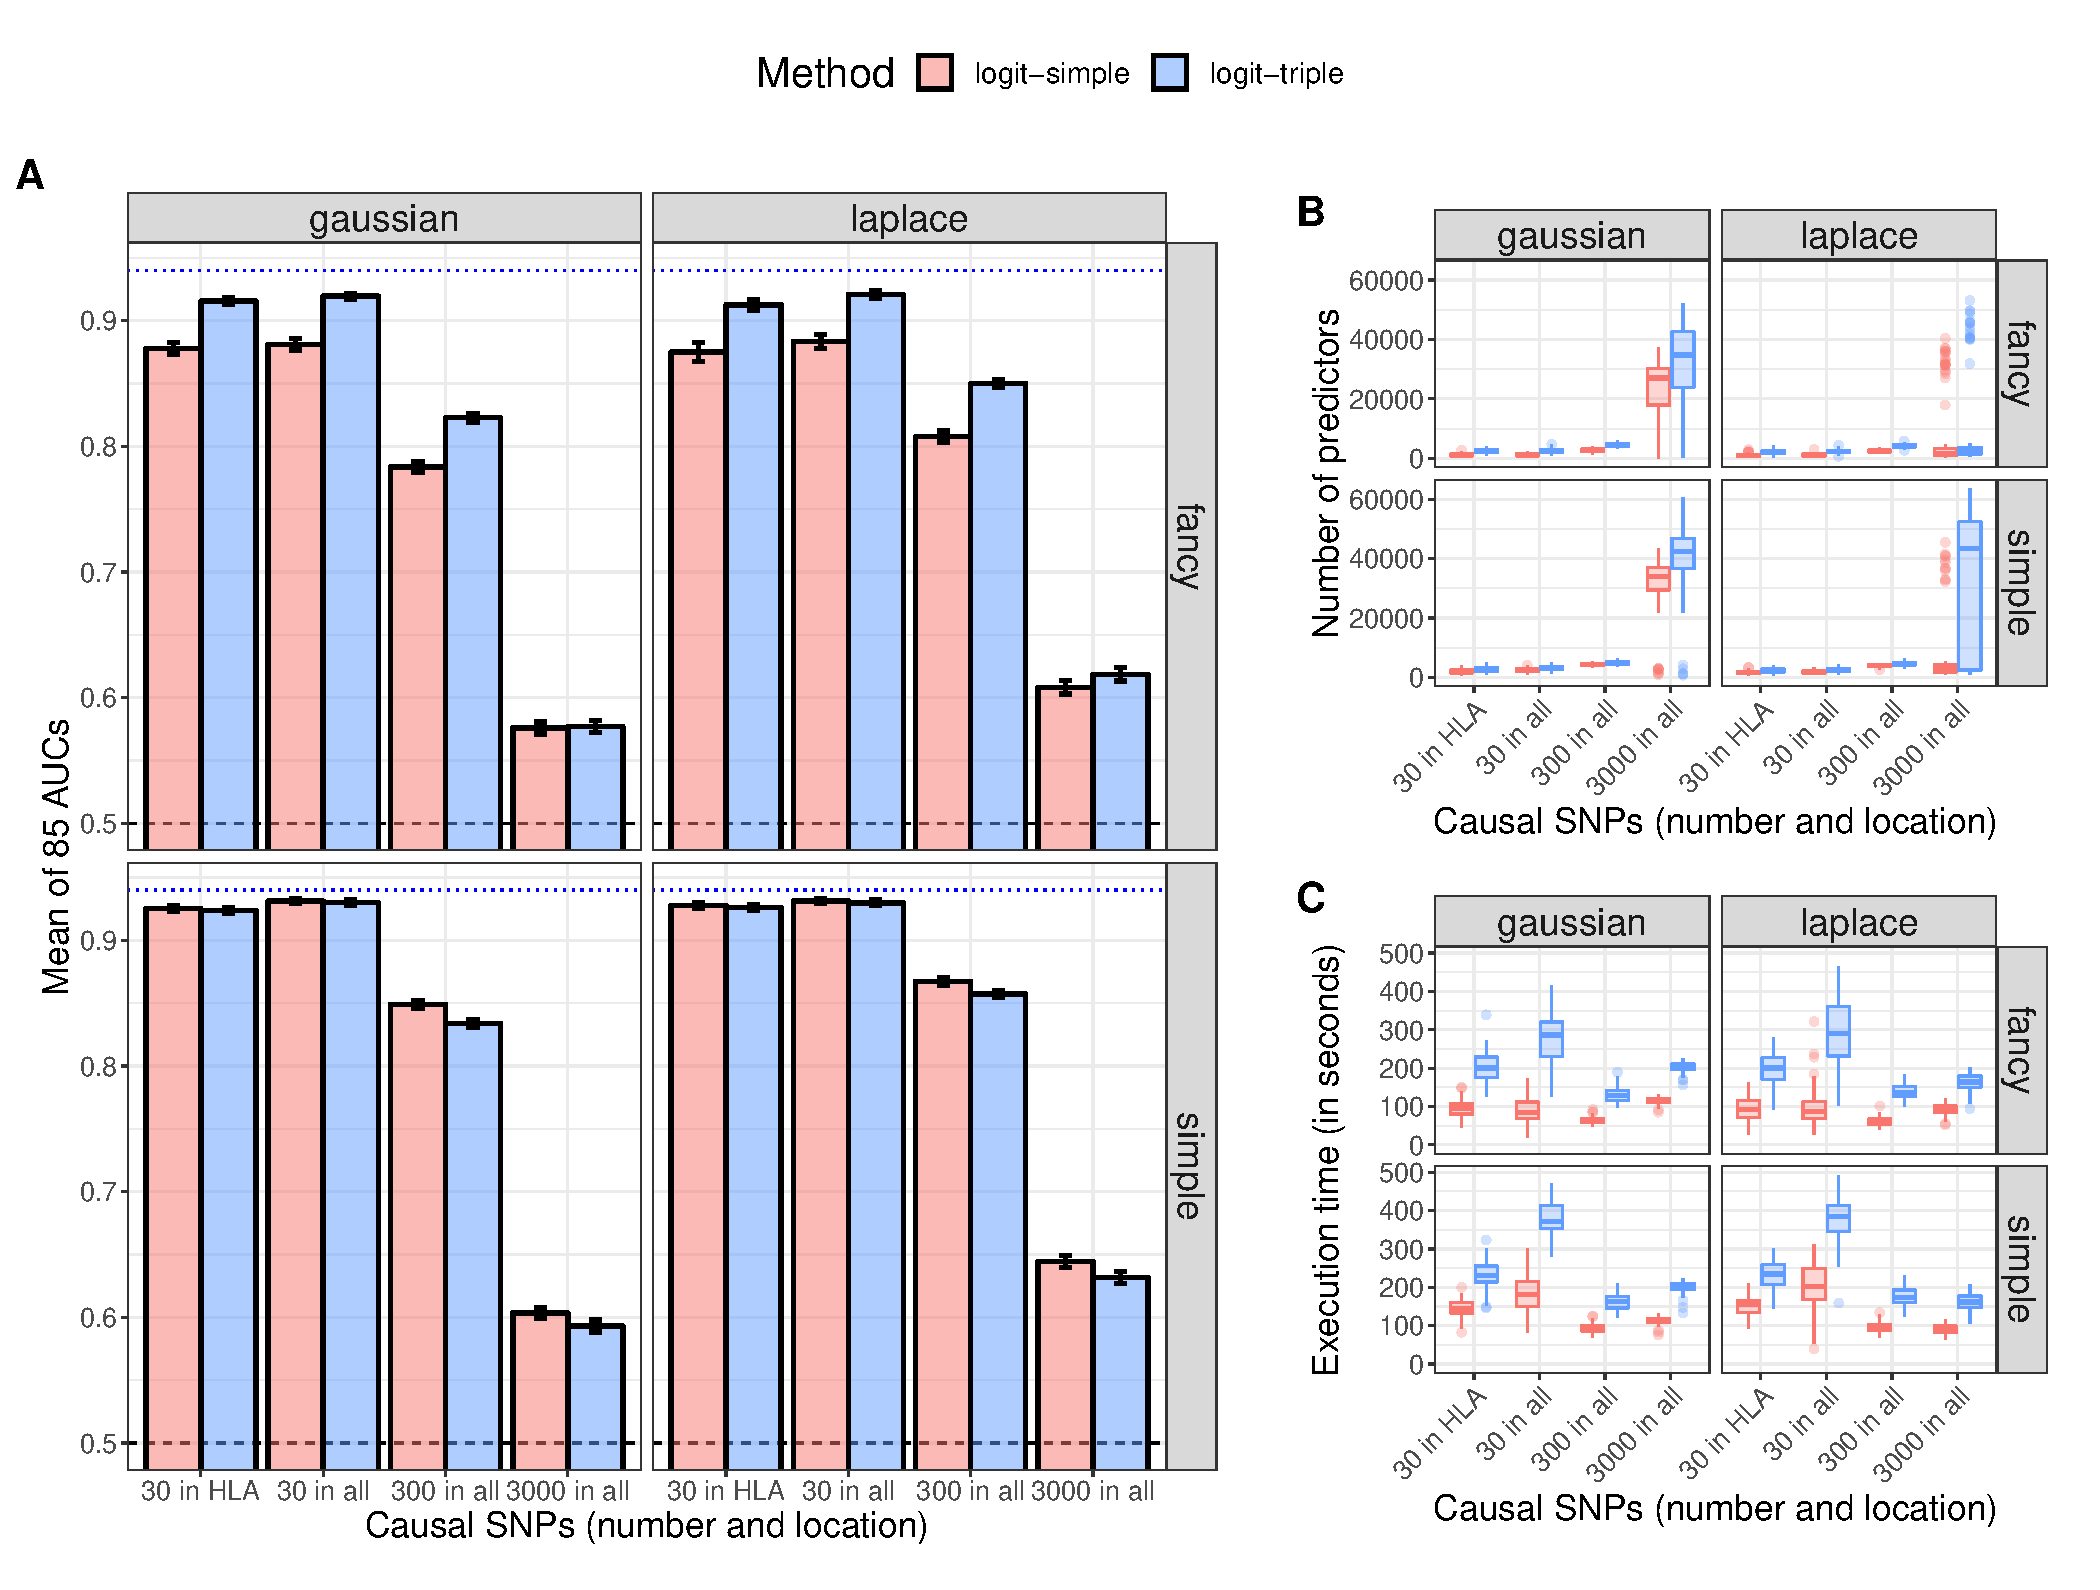
\includegraphics[width=\textwidth]{supp-triple}}
\caption{Comparison of ``logit-triple'' and ``logit-simple'' in scenario \textnumero1 for an heritability of 80\%. Vertical panels are presenting results for effects following a Gaussian or Laplace distribution. Horizontal panels are presenting results for the ``simple'' and ``fancy'' models for simulating phenotypes. \textbf{A:} Mean of AUC over 100 simulations. Error bars are representing $\pm 2 \text{SD}$ of $10^5$ non-parametric bootstrap of the mean of AUC. The blue dotted line represents the maximum achievable AUC. \textbf{B:} Boxplots of numbers of predictors used by the methods for 100 simulations. \textbf{C:} Boxplots of execution times for 100 simulations.}
\label{fig:supp-triple}
\end{figure}


\newpage
\begin{figure}[h]
\centerline{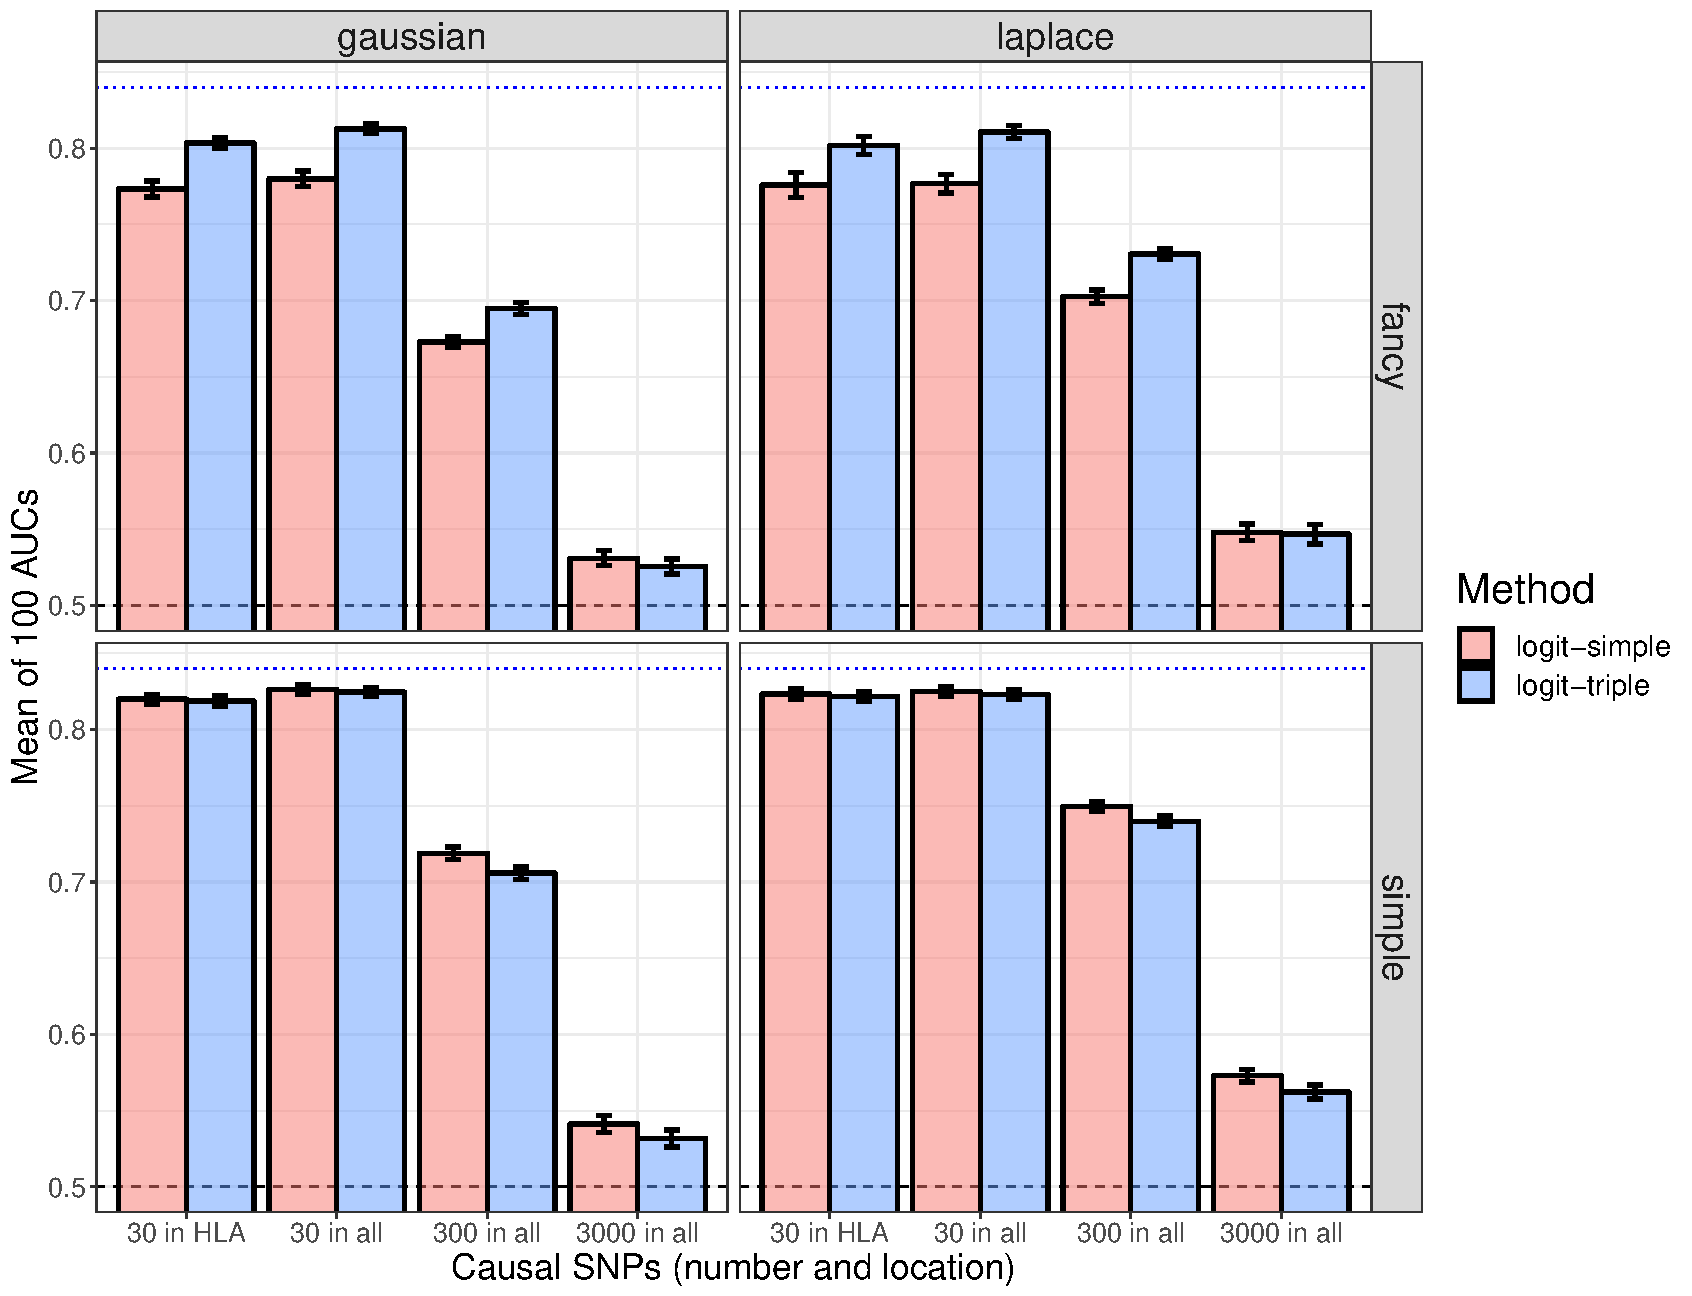
\includegraphics[width=\textwidth]{supp-AUC-triple}}
\caption{Comparison of ``logit-triple'' and ``logit-simple'' in scenario \textnumero1 for an heritability of 50\%. Vertical panels are presenting results for effects following a Gaussian or Laplace distribution. Horizontal panels are presenting results for the ``simple'' and ``fancy'' models for simulating phenotypes. \textbf{A:} Mean of AUC over 100 simulations. Error bars are representing $\pm 2 \text{SD}$ of $10^5$ non-parametric bootstrap of the mean of AUC. The blue dotted line represents the maximum achievable AUC.}
\label{fig:supp-AUC-triple}
\end{figure}

%%%%%%%%%%%%%%%%%%%%%%%%%%%%%%%%%%%%%%%%%%%%%%%%%%%%%%%%%%%%%%%%%%%%%%%%%%%%%%%%

\newpage
\begin{figure}[h]
\centerline{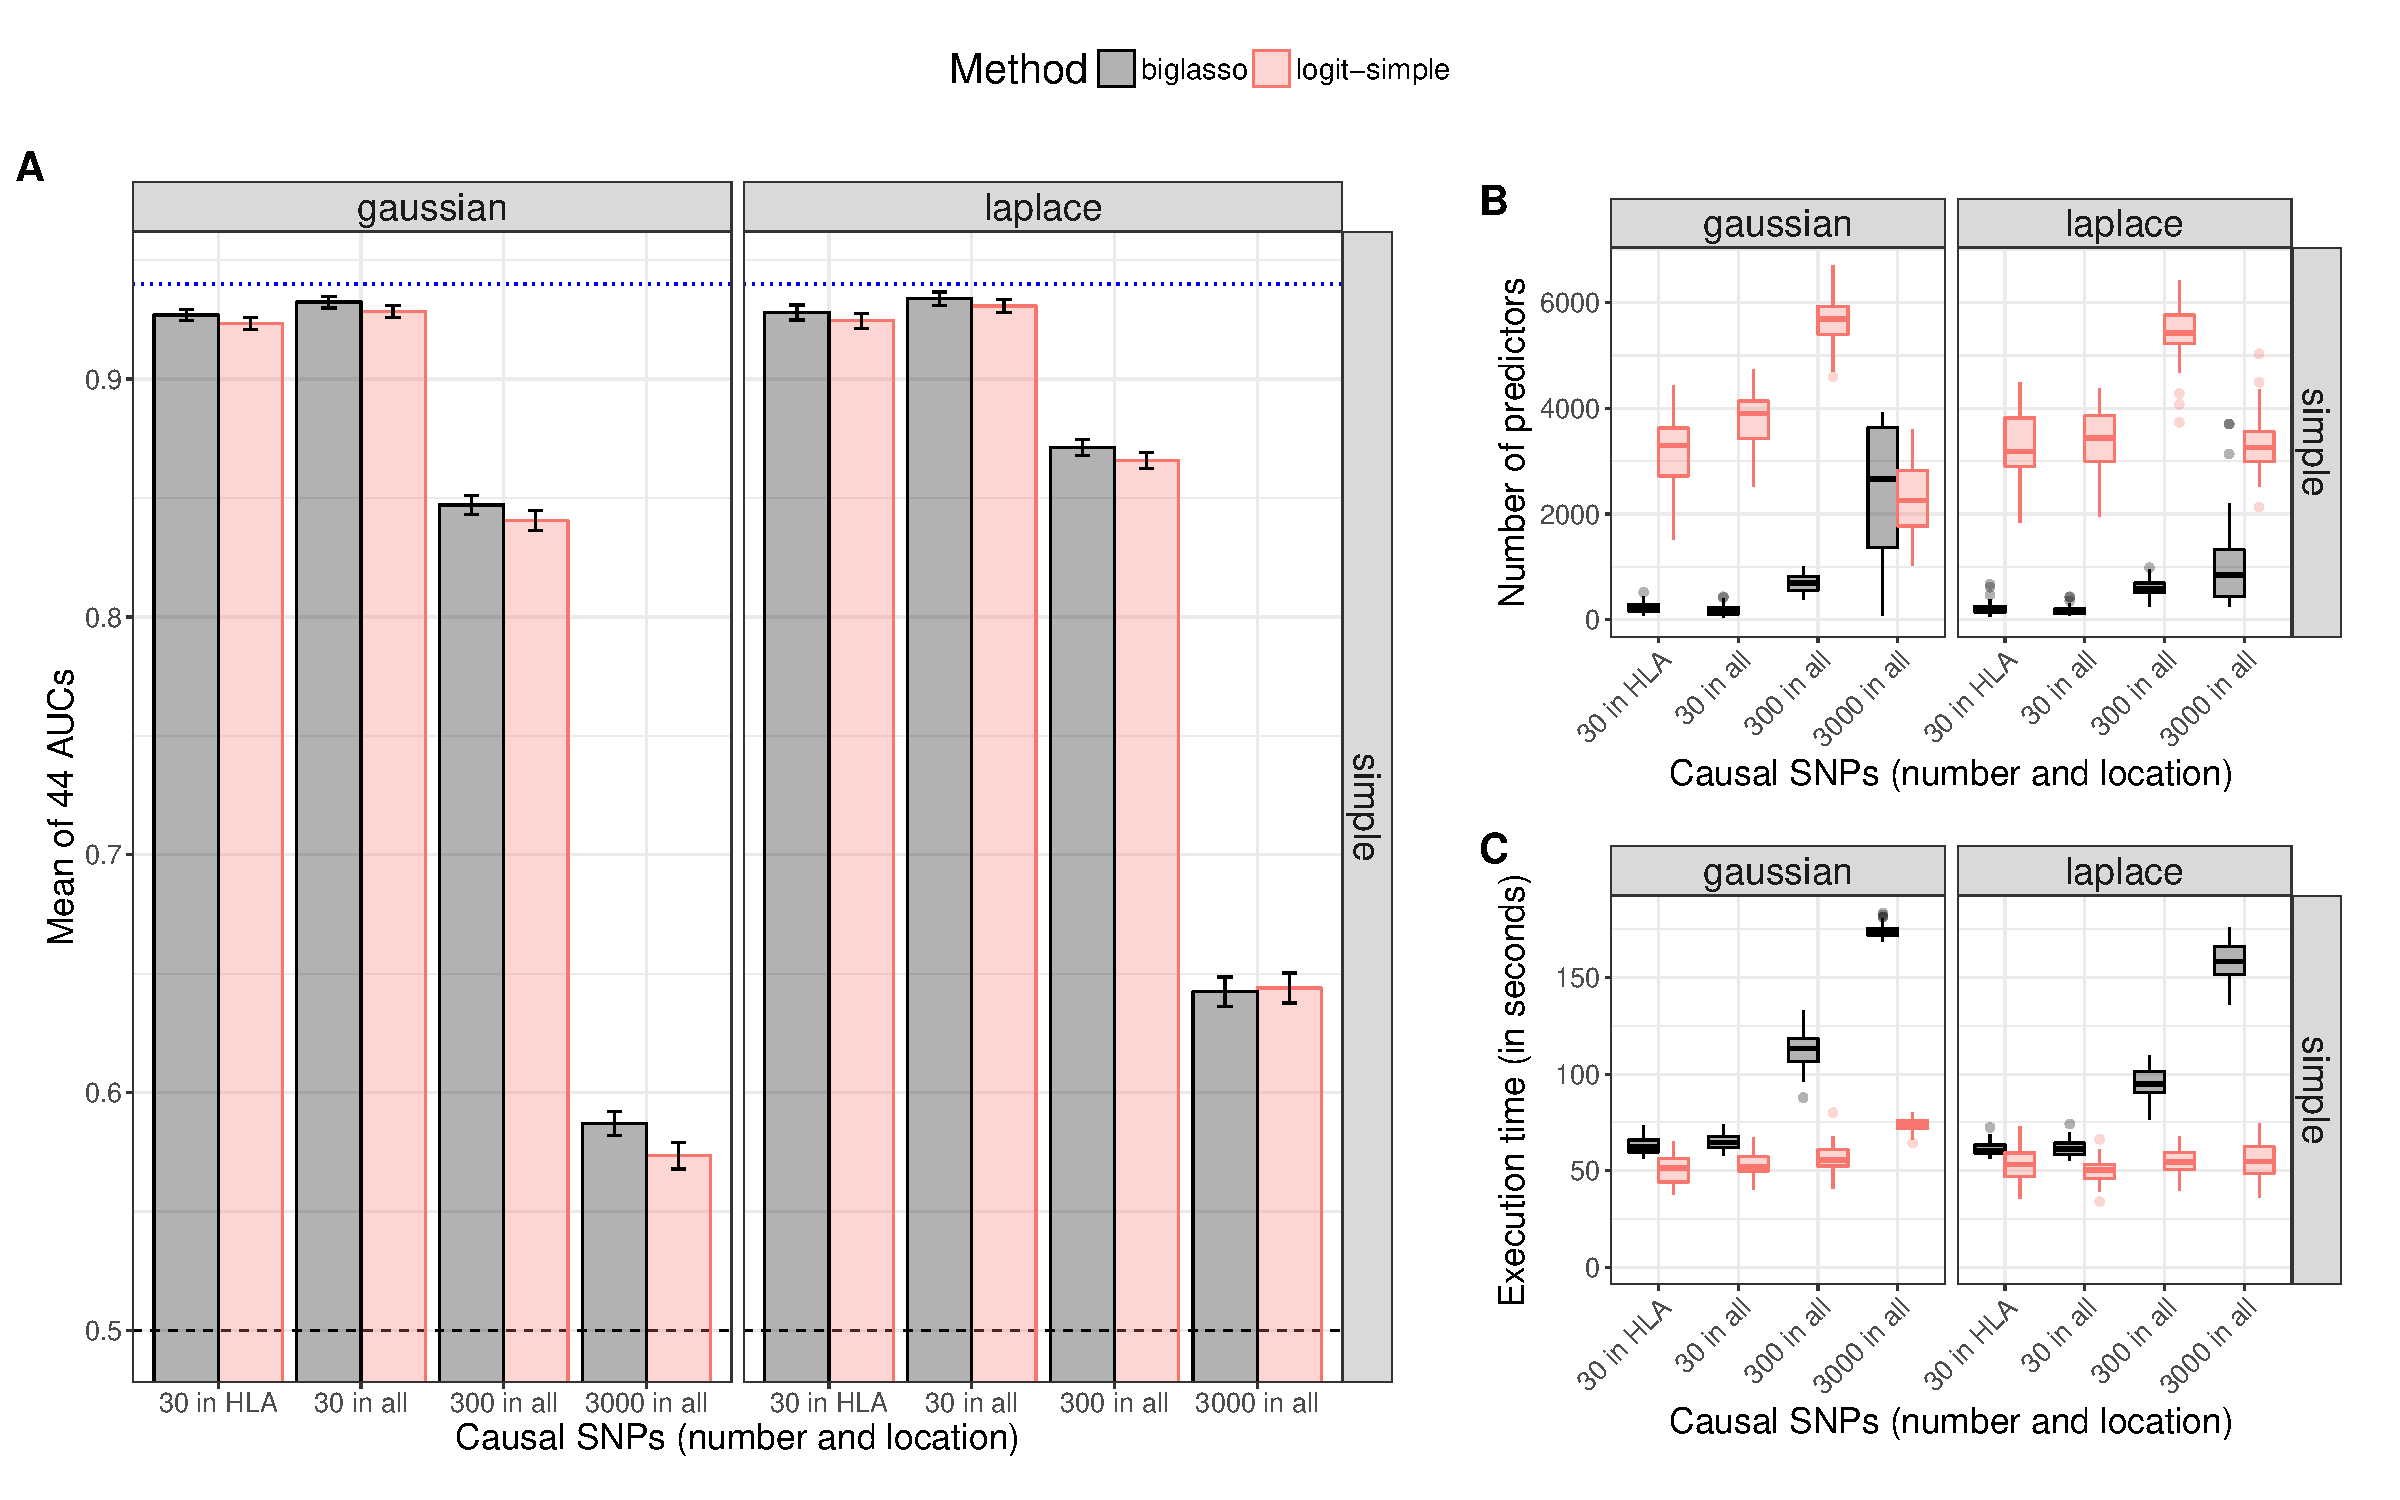
\includegraphics[width=\textwidth]{supp-biglasso}}
\caption{Comparison of ``logit-triple'' and the best prediction (among 100 tested $\lambda$ values) for ``biglasso'' (another implementation of penalized logistic regression) in scenario \textnumero1. Simulations use the ``simple'' model, an heritability of 80\% and $\alpha = 1$. Vertical panels are presenting results for effects following a Gaussian or Laplace distribution. \textbf{A:} Mean of AUC over 100 simulations. Error bars are representing $\pm 2 \text{SD}$ of $10^5$ non-parametric bootstrap of the mean of AUC. The blue dotted line represents the maximum achievable AUC. \textbf{B:} Boxplots of numbers of predictors used by the methods for 100 simulations. \textbf{C:} Boxplots of execution times for 100 simulations.}
\label{fig:supp-biglasso}
\end{figure}

%%%%%%%%%%%%%%%%%%%%%%%%%%%%%%%%%%%%%%%%%%%%%%%%%%%%%%%%%%%%%%%%%%%%%%%%%%%%%%%%


\end{document}
